\subsection{OSG View}
\label{sec:osgview}

The OSG View allows a graphical representation of target reports from the Database Objects. After creation, it displays a world map in the map widget on the left, supported by a configuration panel on the right hand side.

\begin{figure}[H]
    \hspace*{-2cm}
    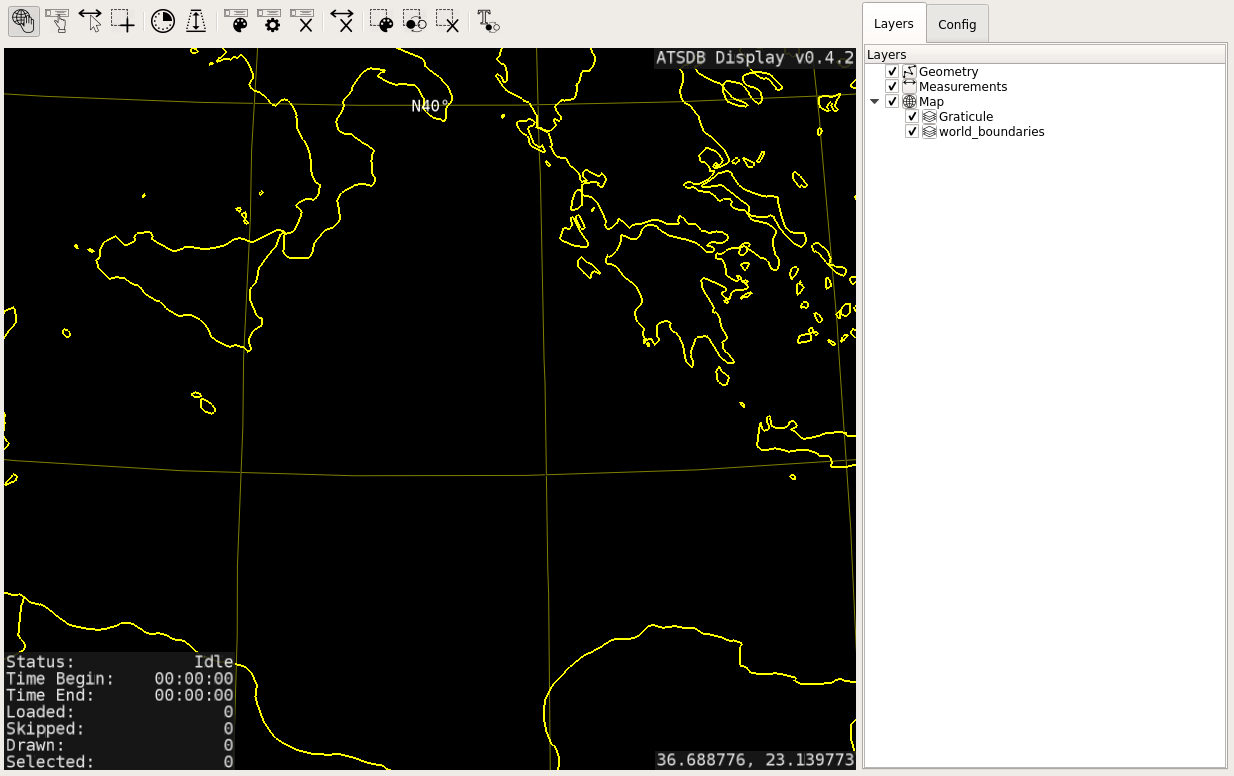
\includegraphics[width=18cm,frame]{../screenshots/osgview_overview.png}
  \caption{OSG View overview}
  \label{fig:osgview_overview}
\end{figure}

The map window will automatically traverse to the medium location of the data in the current database.

After loading, the target reports will be shown.

\begin{figure}[H]
    \hspace*{-2cm}
    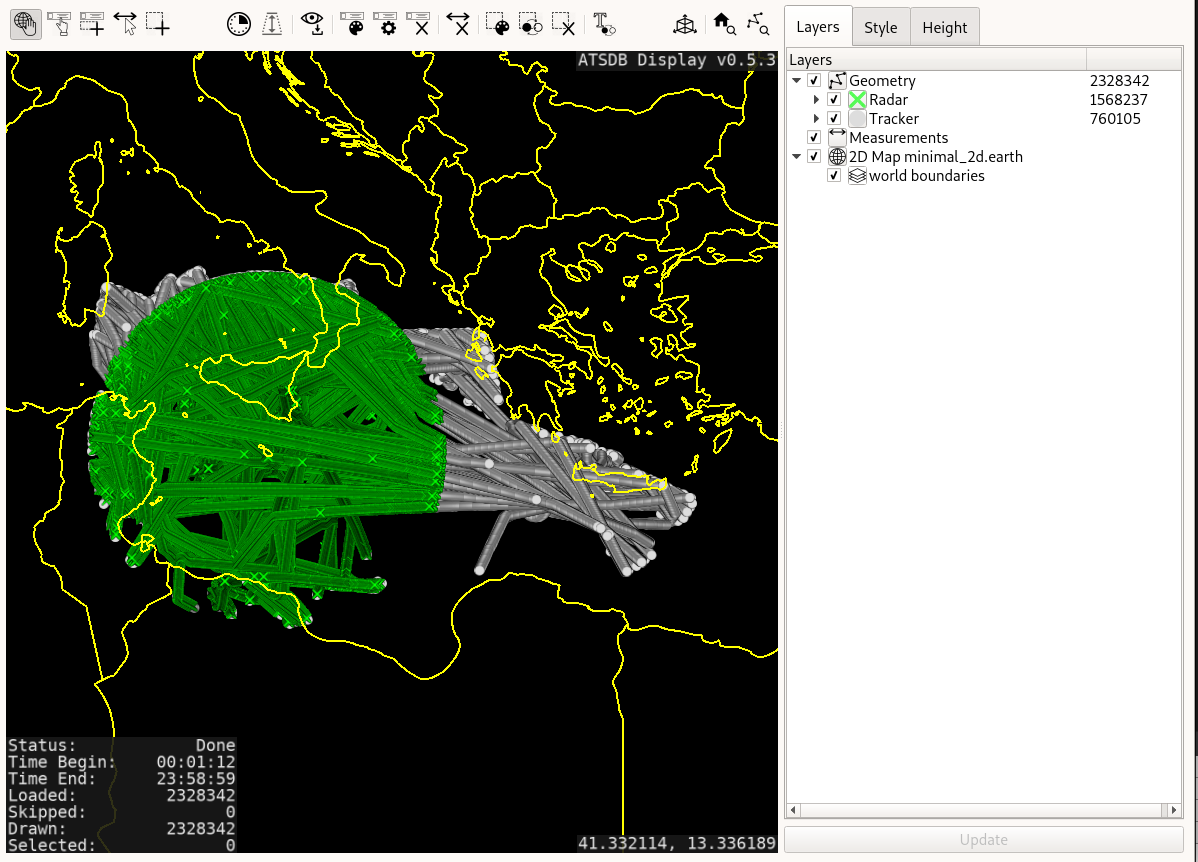
\includegraphics[width=18cm,frame]{../screenshots/osgview_overview_loaded.png}
  \caption{OSG View overview after loading}
\end{figure}

There exist 3 main components:
\begin{itemize}
 \item Toolbar (top left): Selects mouse action or set display options.
 \item Map Widget (lower left): Displays map and geometry data.
 \item Configuration Widget (right): Displays layer selections and set height configuration.
\end{itemize}

\subsubsection{Toolbar}

The first 3 symbols switch between the mouse action modes, the others provide specific options.

\begin{table}[H]
  \center
  \begin{tabular}{ | l | l | l |}
    \hline
    \textbf{Icon} & \textbf{Text} &  \textbf{Description} \\ \hline
    
\includegraphics[width=0.5cm]{../../data/icons/navigate.png} & Navigate & Allows navigation of the map only \\ \hline
    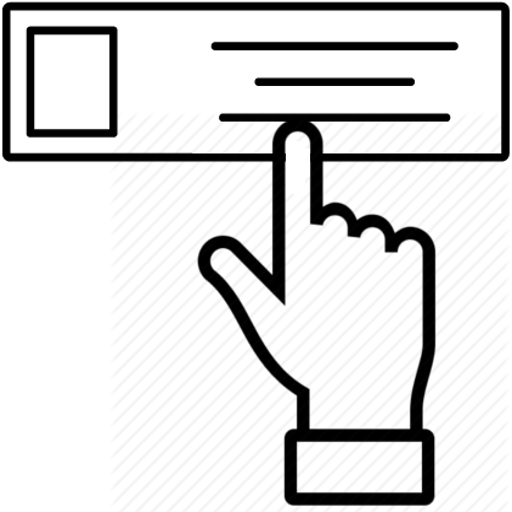
\includegraphics[width=0.5cm]{../../data/icons/label_action.png} & Label & Allows labeling, group menu and nagivation of the map \\ \hline
    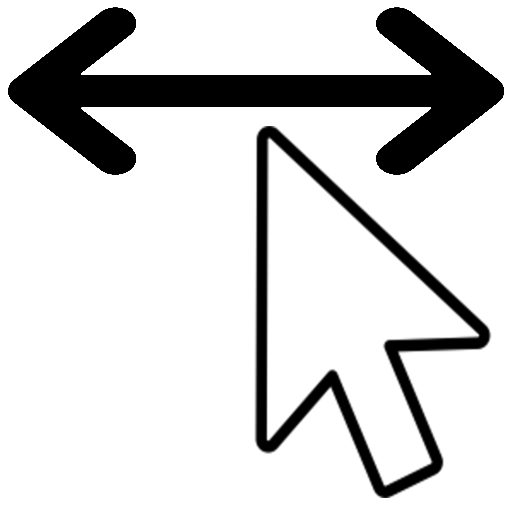
\includegraphics[width=0.5cm]{../../data/icons/measure_action.png} & Measure & Allows map distance measuring and navigation of the map \\ \hline
    
\includegraphics[width=0.5cm]{../../data/icons/select_action.png} & Select & Allows data selection \& de-selection \\ \hline
  \end{tabular}
  \caption{Toolbar mouse action modes}
\end{table}

The others provide general display modes or operations.

\begin{table}[H]
  \center
  \begin{tabular}{ | l | l | l |}
    \hline
    \textbf{Icon} & \textbf{Text} &  \textbf{Description} \\ \hline
    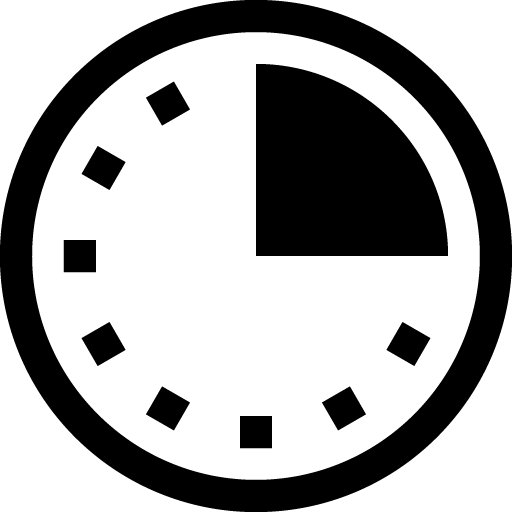
\includegraphics[width=0.5cm]{../../data/icons/time.png} & Toggle Time Filter & Enable/disable time filter \\ \hline
    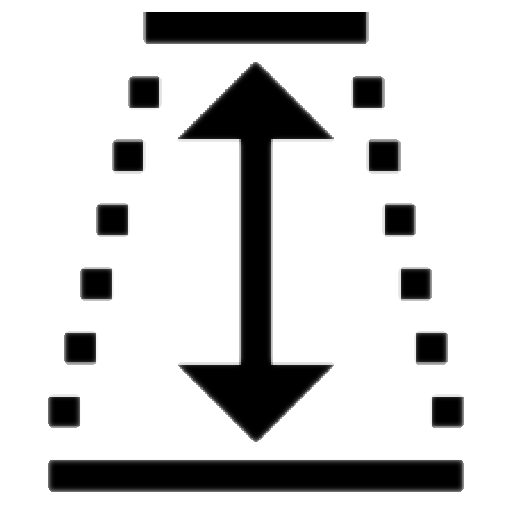
\includegraphics[width=0.5cm]{../../data/icons/depth.png} & Toggle Depth Check & Enable/disable depth check \\ \hline
    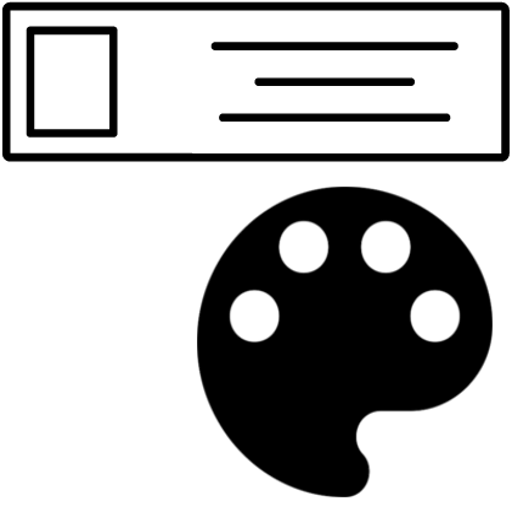
\includegraphics[width=0.5cm]{../../data/icons/label_color.png} & Edit Label Color & Set background color for all labels \\ \hline
    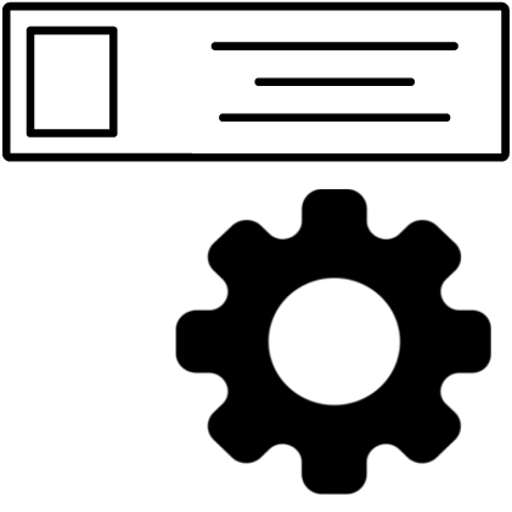
\includegraphics[width=0.5cm]{../../data/icons/label_edit.png} & Edit Label Content & Edit the content for labels \\ \hline
    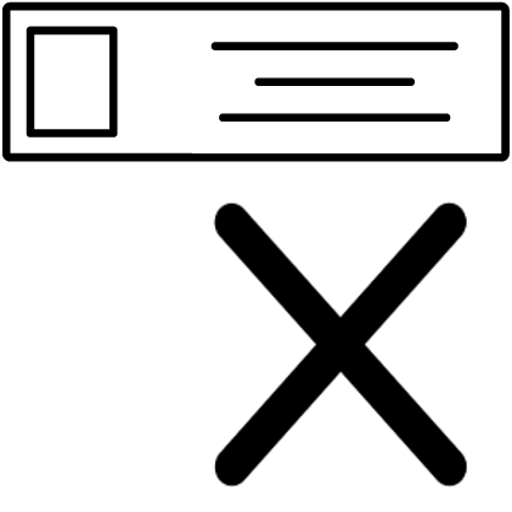
\includegraphics[width=0.5cm]{../../data/icons/label_delete.png} & Deletes All Labels & Deletes all existing labels \\ \hline
    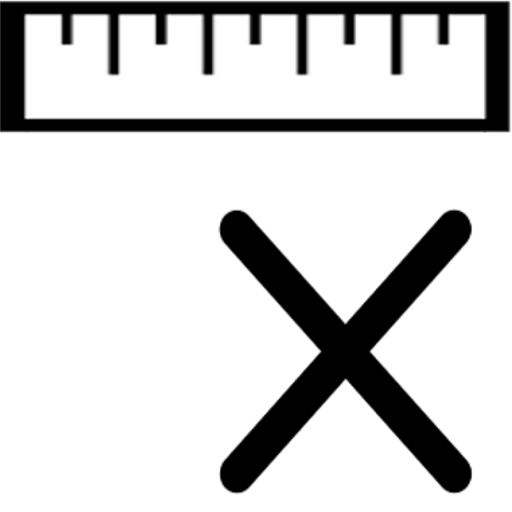
\includegraphics[width=0.5cm]{../../data/icons/measurement_delete.png} & Deletes All Measurements & Deletes all existing measurements \\ \hline 
\includegraphics[width=0.5cm]{../../data/icons/select_color.png} & Edit Selection Color & Set selection color \\ \hline
    
\includegraphics[width=0.5cm]{../../data/icons/select_invert.png} & Invert Selection & Selects all de-selected \& vice versa \\ \hline
    
\includegraphics[width=0.5cm]{../../data/icons/select_delete.png} & Delete Selection & De-selects all target reports \\ \hline
    
\includegraphics[width=0.5cm]{../../data/icons/text_invert.png} & Overlay Text Color Invert & Changes Overlay Text Color \\ \hline
  \end{tabular}
  \caption{Toolbar operations}
\end{table}


\subsubsection{Map Widget}
\label{sec:osgview_map}

In the map widget, several mouse and key operations are supported. The following terms are used:

\begin{itemize}
 \item LMB: Left mouse button
 \item MMB: Middle mouse button
 \item RMB: Right mouse button
\end{itemize}

The following operations exist, depending on the mouse action modes:

\begin{table}[H]
  \center
  \begin{tabular}{ | l | l | l |}
    \hline
    \textbf{Mouse Action} & \textbf{Key Action} &  \textbf{Description} \\ \hline
    LMB click & - & - \\ \hline
    LMB click \& drag & - & Traverse map \\ \hline
    LMB double click & - & Zoom to clicked location \\ \hline
    - & Arrows & Traverse map \\ \hline
    MMB click \& drag & - & Rotate map \\ \hline
    MMB scroll \& drag & - & Zoom map \\ \hline
    RMB click & - & - \\ \hline
    RMB click \& drag & - & Zoom map \\ \hline
    RMB double click \& drag & - & Zoom away from clicked location \\ \hline
    - & Space bar & Return to home position \\ \hline
  \end{tabular}
  \caption{Map widget view operations in Navigate mode}
\end{table}

\begin{table}[H]
  \center
  \begin{tabular}{ | l | l | l |}
    \hline
    \textbf{Mouse Action} & \textbf{Key Action} &  \textbf{Description} \\ \hline
    LMB click & - & Create label \\ \hline
    LMB click \& drag & - & Create label \& traverse map \\ \hline
    RMB click & - & Open group menu \\ \hline
    ... & ... & Other operations are the same as in Navigate mode \\ \hline
  \end{tabular}
  \caption{Map widget view operations in Label mode}
\end{table}

\begin{table}[H]
  \center
  \begin{tabular}{ | l | l | l |}
    \hline
    \textbf{Mouse Action} & \textbf{Key Action} &  \textbf{Description} \\ \hline
    LMB click & - & Start/end measurement \\ \hline
    LMB click \& drag & - & Traverse map \\ \hline
    ... & ... & Other operations are the same as in Navigate mode \\ \hline  
    \end{tabular}
  \caption{Map widget view operations in Measure mode}
\end{table}

\begin{table}[H]
  \center
  \begin{tabular}{ | l | l | l |}
    \hline
    \textbf{Mouse Action} & \textbf{Key Action} &  \textbf{Description} \\ \hline
    LMB click & - & Start/end selection box \\ \hline
    LMB click \& drag & - & Traverse map \\ \hline
    ... & ... & Other operations are the same as in Navigate mode \\ \hline  
    \end{tabular}
  \caption{Map widget view operations in Select mode}
\end{table}

Further operations are defined in section Map Widget Data Operations. \\

In the lower-left corner, the data status information is given:

\begin{itemize}
 \item Status
\begin{itemize}
 \item Idle: Nothing to do
 \item Loading: Loading in progress
 \item Done: Loading/redraw done
 \item Redrawing: Redraw in progress
\end{itemize}
 \item Time Begin: First timestamp in the data, in HH:MM:SS
 \item Time End: last timestamp in the data, in HH:MM:SS
 \item Loaded: Number of loaded target reports (from the database)
 \item Skipped: Number of not-drawn target reports
 \item Drawn: Number of drawn target reports
 \item Selected: Number of selected target reports
\end{itemize}

In the upper-right corner, the ATSDB version is shown. In the lower-right corner, the current coordinates (map coordinates under the mouse cursor) are shown.

\subsubsection{Configuration Widget}
\label{sec:osgview_config}

In the configuration widget, several elements exist:

\begin{itemize}
 \item Layer widget: displays all currently existing layers
 \item Configuration area
\begin{itemize}
 \item Group Variable: Meta DBOVariable used to create groups. Currently, only track number and Mode S address are supported
 \item Connect groups: Whether grouped target reports should be connected using lines
 \item Connect None Height: If groups are connected, whether target reports with not height information should be connected
 \item Use Height: Whether height information should be used to create a 3D presentation
 \item Offset Factor: If height information is used, this factor is added to the height
 \item Scale Factor: If height information is used, this factor is used to multiply the height
 \item Null Offset: If height information is used, this factor is used for target reports without height information
 \item Redraw button: Triggers a re-draw of the geometry, e.g. after a one of the above options was used
\end{itemize}
\end{itemize}

\subsubsection{Layer Widget}

In the layer widget, a tree view is given to configure the display of the existing elements. The following main tree elements are:
\begin{itemize}
 \item Geometry: Shows current DBO elements
 \item Measurements: Shows the current distance measurements
 \item Map: Shows current map layers
\end{itemize}

\subsubsection{Changing the Background Map}

Please note that, while the default background map is supplied ATSDB, the other background map types are downloaded from public Internet sources and therefore require an Internet connection. They are then cached locally to facilitate faster access. \\

For each map layer defined in the background map, a checkbox is shown to disable the layer, and by clicking on the map layer symbol it's opacity can be changed.

To change the background map, click the globe symbol {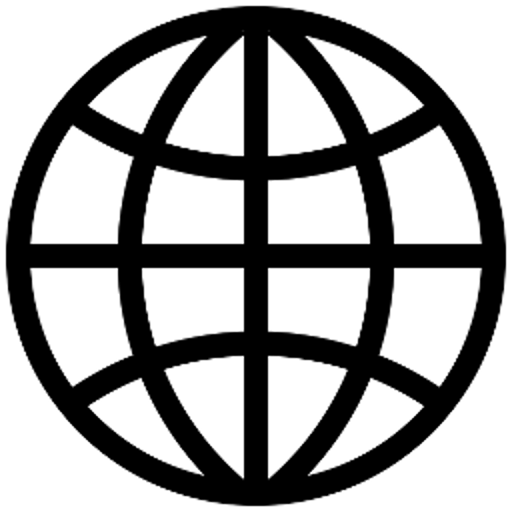
\includegraphics[width=0.5cm]{../../data/icons/globe.png} in root Map layer to access the map selection. The following maps are commonly available:

\begin{itemize}
 \item arcgis.earth
 \item minimal\_new.earth
 \item openstreetmap.earth
 \item readymap.earth
 \item readymap-detailed.earth
\end{itemize}

The map loading and display in based on the osgEarth library (\url{http://osgearth.org/}), as are to map file definitions.  \\

The map which can be set using this dialog is simply a file list from the folder '\textasciitilde/.atsdb/data/maps'. So, changes can be made to the supplied ones or custom user maps can be added to this folder. \\
Please refer to section \nameref{sec:adding_maps} for further details.

\newpage
\paragraph{ArcGIS Map}

As supplied in the osgEarth example files, this map data is obtained from ArcGIS Online (\url{https://doc.arcgis.com/en/arcgis-online/reference/what-is-agol.htm}). It shows satellite imagery, supplied with elevation data from ReadyMap. 

\begin{figure}[H]
    \hspace*{-2cm}
    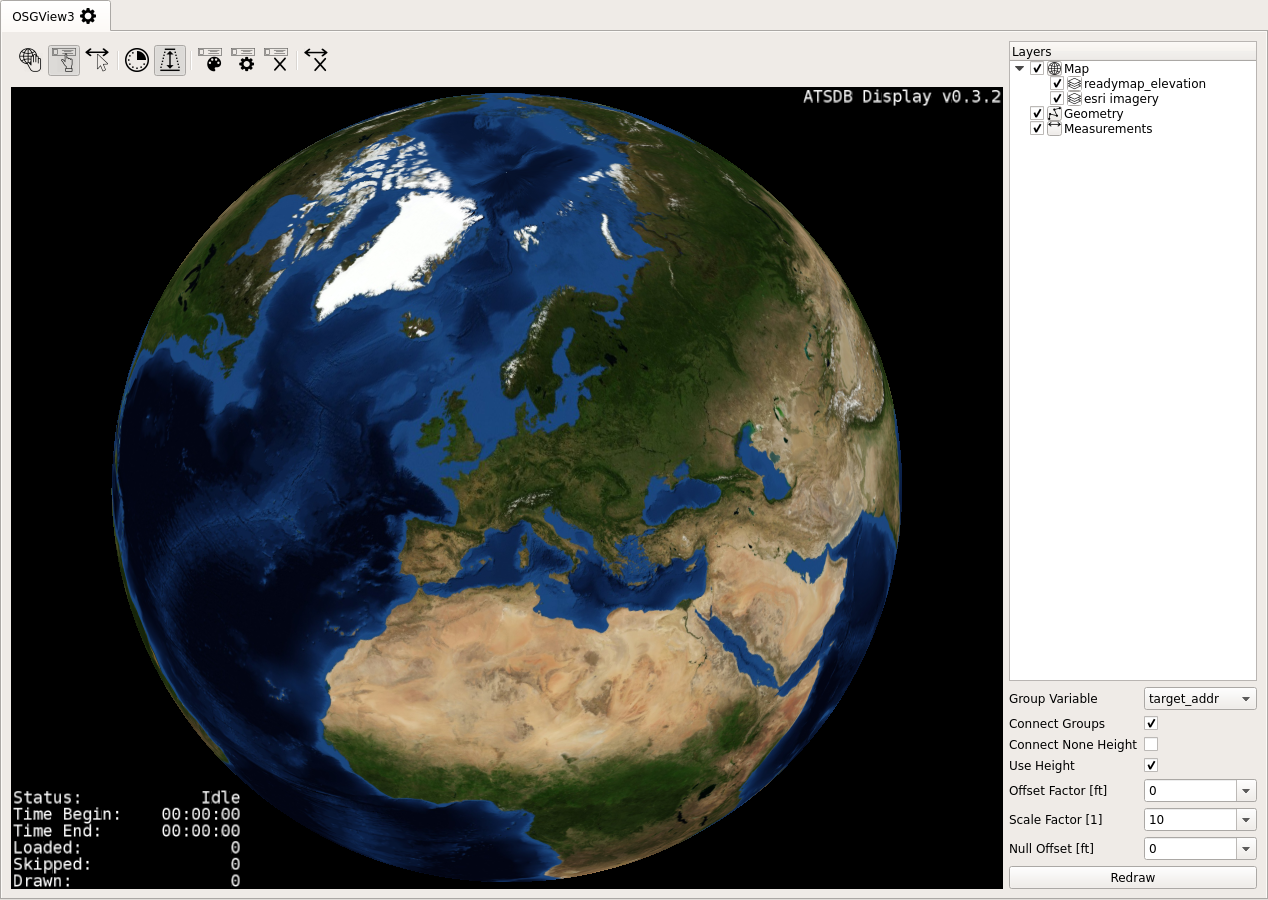
\includegraphics[width=18cm,frame]{../screenshots/osgview_arcgis.png}
  \caption{OSG View Arcgis map}
\end{figure}

\newpage
\paragraph{Minimal Map}

This minimal map shows national borders based on an ESRI shapefile, provided by Bjorn Sandvik on \url{thematicmapping.org}. In the AppImage application the 'minimal\_new.earth' file should be used.

\begin{figure}[H]
    \hspace*{-2cm}
    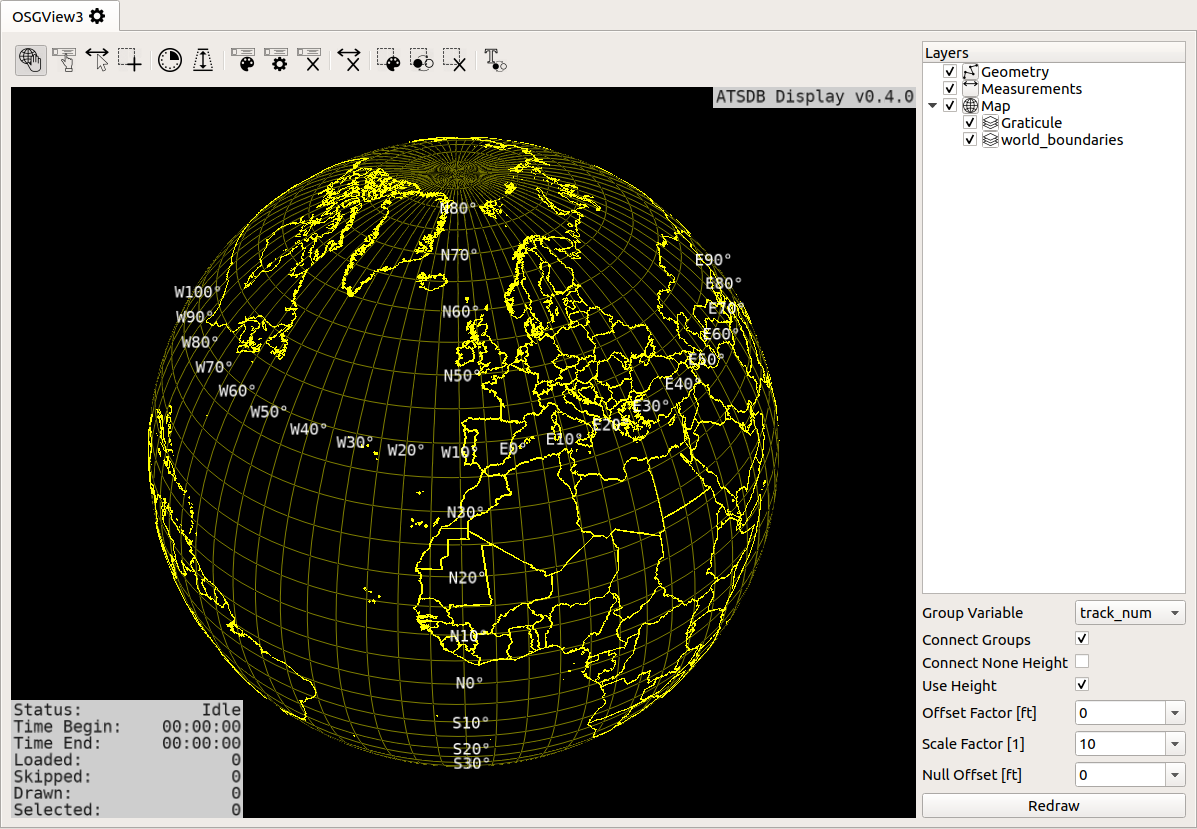
\includegraphics[width=18cm,frame]{../screenshots/osgview_minimal.png}
  \caption{OSG View minimal map}
\end{figure}

\newpage
\paragraph{Open Street Map}

This very useful map shows map data from \url{https://www.openstreetmap.org/}.

\begin{figure}[H]
    \hspace*{-2cm}
    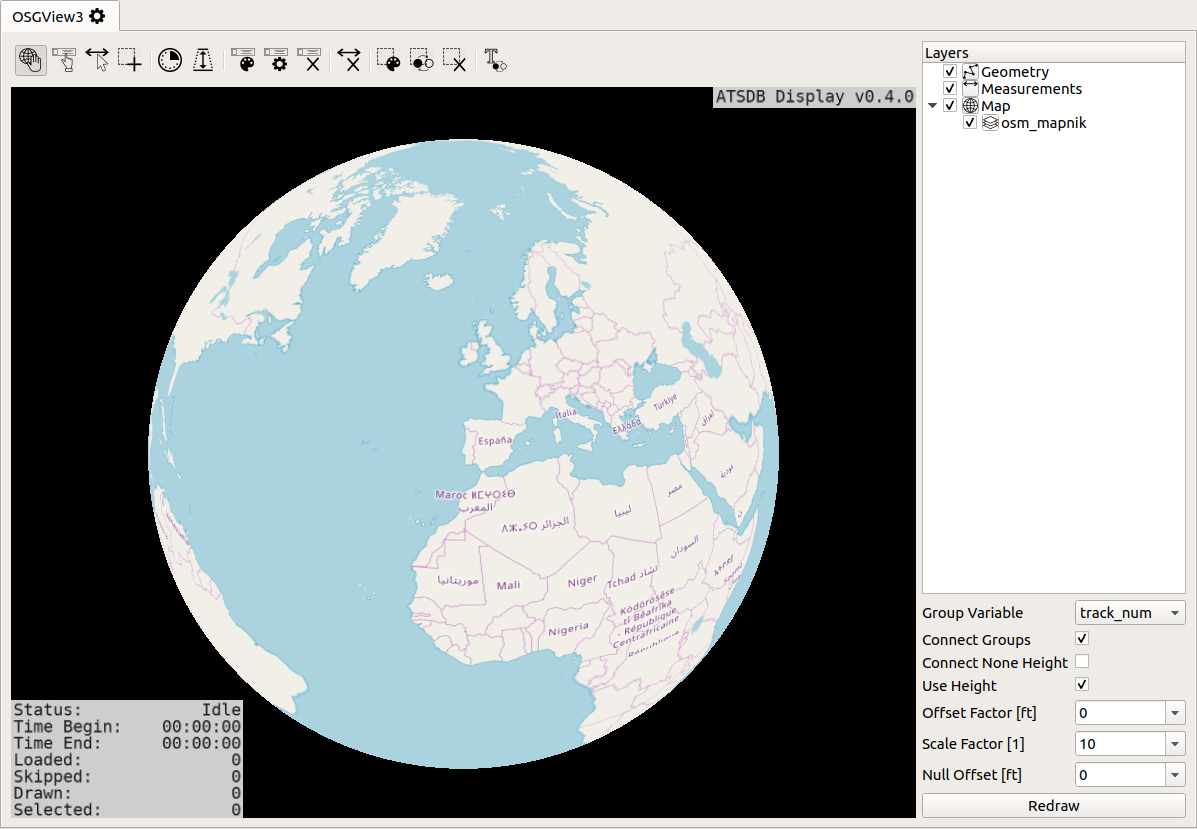
\includegraphics[width=18cm,frame]{../screenshots/osgview_osm.png}
  \caption{OSG View OpenStreetMap}
\end{figure}

It is possible to zoom in to a very high level of detail, to even inspect airport layouts.

\begin{figure}[H]
    \hspace*{-2cm}
    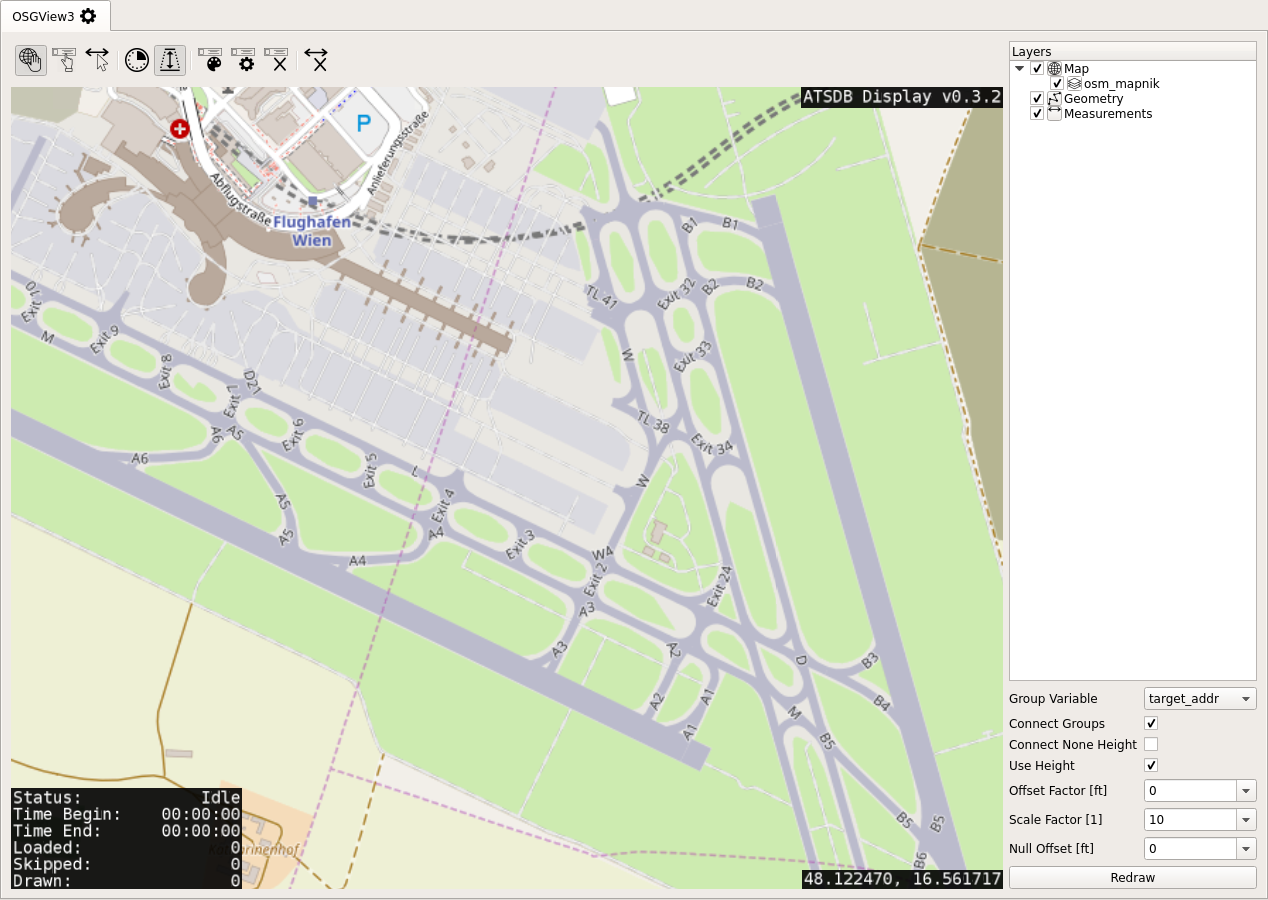
\includegraphics[width=18cm,frame]{../screenshots/osgview_osm_vienna.png}
  \caption{OSG View OpenStreetMap Vienna Airport}
\end{figure}

\newpage
\paragraph{ReadyMap}

This map also shows satellite data, from \url{http://web.pelicanmapping.com/readymap-tiles/}. It includes an elevation layer, so ground elevation is observable.

\begin{figure}[H]
    \hspace*{-2cm}
    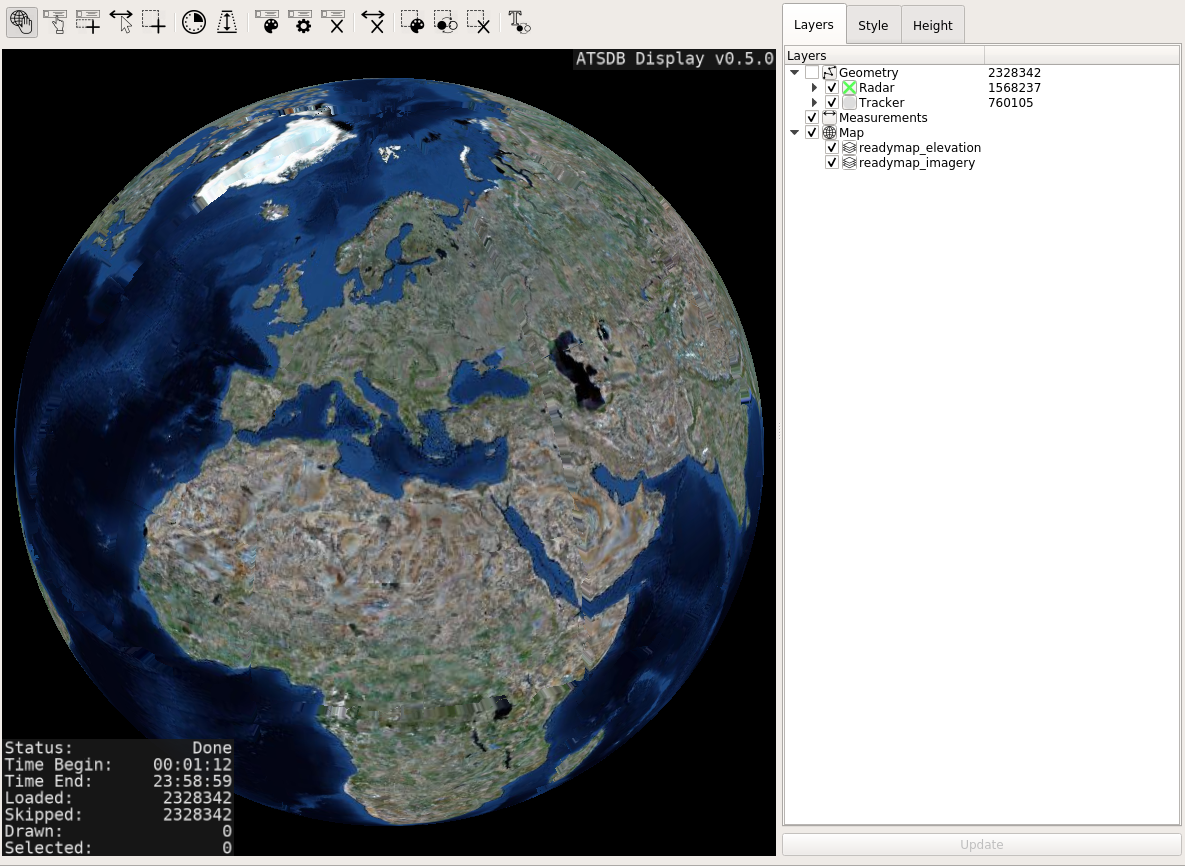
\includegraphics[width=18cm,frame]{../screenshots/osgview_ready.png}
  \caption{OSG View ReadyMap}
\end{figure}


\paragraph{ReadyMap Detailed}

This map shows the same data as ReadyMap, but to a higher detail level.

\begin{figure}[H]
    \hspace*{-2cm}
    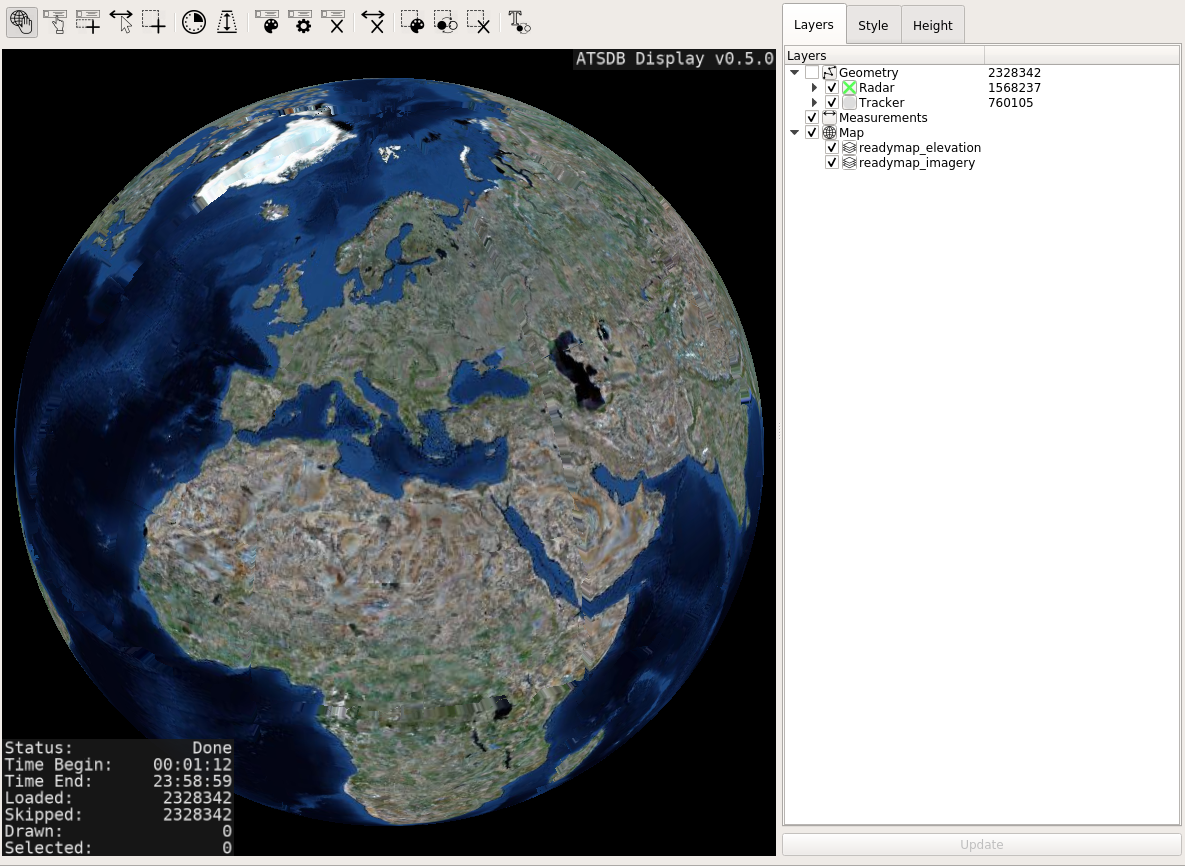
\includegraphics[width=18cm,frame]{../screenshots/osgview_ready.png}
  \caption{OSG View ReadyMap detailed}
\end{figure}

\begin{figure}[H]
    \hspace*{-2cm}
    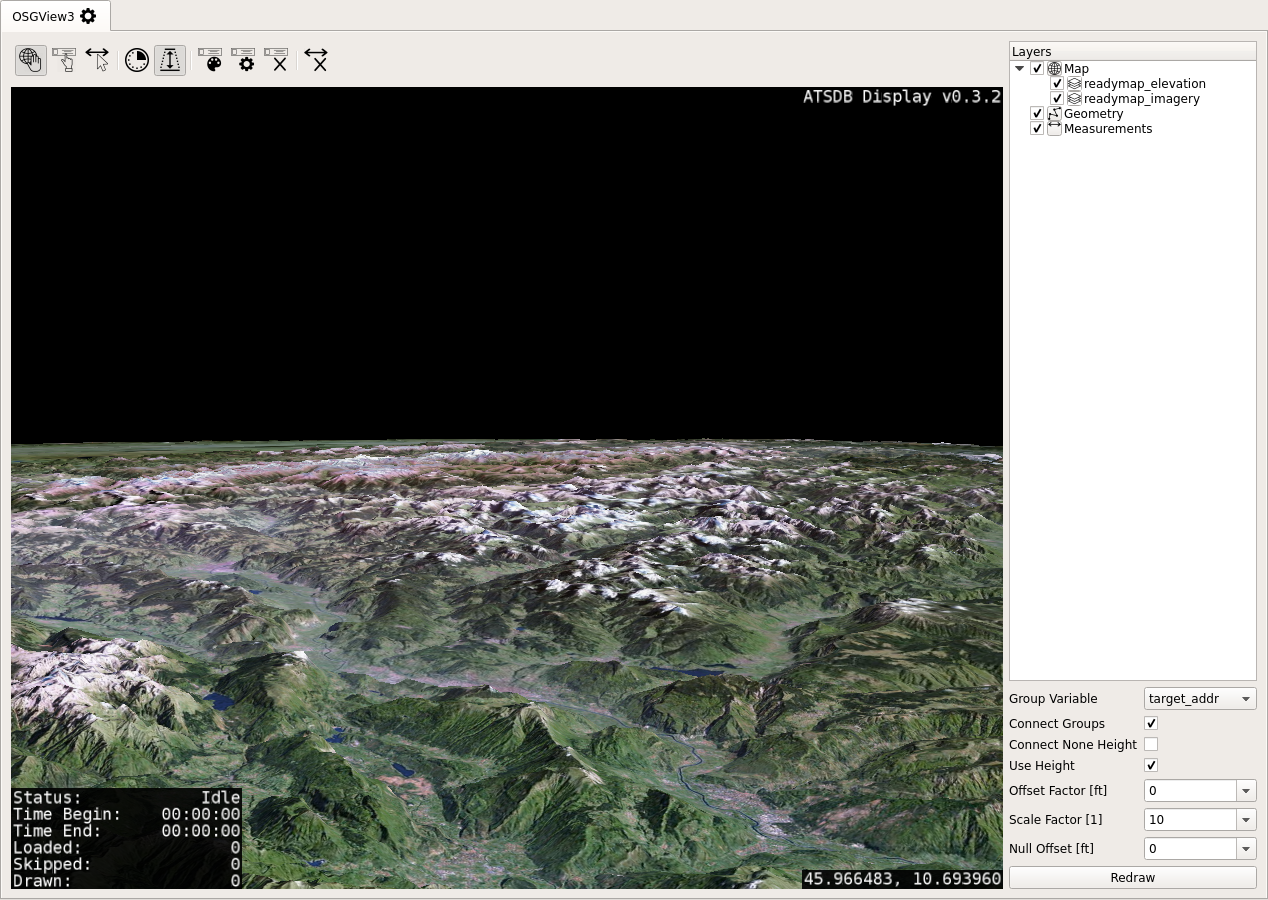
\includegraphics[width=18cm]{../screenshots/osgview_readymap_elav.png}
  \caption{OSG View ReadyMap detailed elevation}
\end{figure}

\subsubsection{Adding/Changing Map Files}
\label{sec:adding_maps}

As with all configuration, a local version is kept in the home folder of the user. The map files are loaded from the hidden folder '\textasciitilde/.atsdb/data/maps' ('\textasciitilde' is the user's home directory, like /home/user).

\begin{figure}[H]
    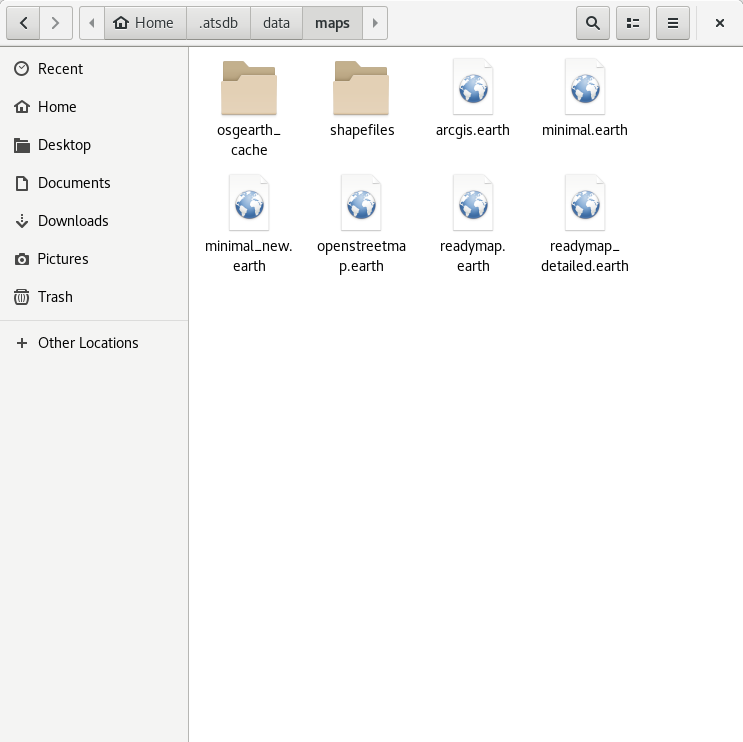
\includegraphics[width=10cm,frame]{../screenshots/maps_config.png}
  \caption{Maps Folder}
\end{figure}

In this folder, the previosly discussed maps exist as osgEarth '.earth' files. If new .earth files are added, or the content of such files is changed, they can be used from the OSGView after a restart.

The easiest example is the 'minimal\_new.earth' file, which uses an ESRI shapefile from the subfolder 'shapefiles' to display the national borders.

\begin{verbatim}
<map name="Wordwide Line Vectors" type="geocentric">
  
    <options>
        <lighting>false</lighting>
        <terrain>
            <min_tile_range_factor>8</min_tile_range_factor>
            <color>#000000FF</color>
        </terrain>
      
    </options>

    <feature_source name="world-data" driver="ogr">
        <url>shapefiles/TM_WORLD_BORDERS-0.3.shp</url>
        <convert type="line"/>
    </feature_source>
    
    <feature_model name="world_boundaries" feature_source="world-data">
        
        <layout tile_size="500000"  paged="true">
            <level max_range="1e10"/>
        </layout>
                
        <styles>
            <style type="text/css">
                world {
                   stroke:                   #ffff00;
                   stroke-width:             2px;
                   stroke-tessellation-size: 1km;
                   render-lighting:          false;
                   altitude-clamping:        none;
                }            
            </style>
        </styles>
        
    </feature_model>
 

</map>
\end{verbatim}

The world background colour is set using the 'terrain color' tag. The name of the shapefile is given using the 'url' tag, the line colour and width is set in the style below. Basically a user can add their own files to the 'shapefiles' folder, and simply duplicate the 'feature\_model' part with their own ESRI shapefiles. This could the look like this:

\begin{verbatim}
<map name="Wordwide Line Vectors" type="geocentric">
  
    <options>
        <lighting>false</lighting>
         <terrain color="#101010ff"/>
    </options>

    <feature_source name="world-data" driver="ogr">
        <url>shapefiles/TM_WORLD_BORDERS-0.3.shp</url>
        <convert type="line"/>
    </feature_source>
    
    <feature_model name="world_boundaries" feature_source="world-data">
        
        <layout tile_size="500000"  paged="true">
            <level max_range="1e10"/>
        </layout>
                
        <styles>
            <style type="text/css">
                world {
                   stroke:                   #ffff00;
                   stroke-width:             2px;
                   stroke-tessellation-size: 1km;
                   render-lighting:          false;
                   altitude-clamping:        none;
                }            
            </style>
        </styles>
        
    </feature_model>
  
    <feature_model name="doi">
        <features name="wolrd" driver="ogr">
            <url>shapefiles/doi.shp</url>
            <build_spatial_index>true</build_spatial_index>
            <ogr_driver>ESRI Shapefile</ogr_driver>
            <convert type="line"/>
        </features>        

        <layout tile_size="500000">
            <level max_range="1e10"/>
        </layout>

        <styles>
            <style type="text/css">
                states {
                   stroke:          #00ff00; 
                   stroke-width:    2px;
                   render-depth-test: false;
                }                    
            </style>
        </styles>        
    </feature_model>
  
</map>
\end{verbatim}

While a number of formats are supported, to add a KML file, add the following part to a 'map' (as previously):

\begin{verbatim}
     <feature_model name="wam_area">
        <features name="wam_area" driver="ogr">
            <url>shapefiles/wam_area.kml</url>
            <ogr_driver>LIBKML</ogr_driver>
            <build_spatial_index>true</build_spatial_index>
        </features>        

        <styles>
            <style type="text/css">
                states {
                   stroke:          #0000ff; 
                   stroke-width:    2px;
                   render-depth-test: false;
                }                    
            </style>
        </styles>        
    </feature_model>
\end{verbatim}

To add a GML file, add the following part to a 'map' (as previously):

\begin{verbatim}
   <model driver="feature_geom" name="gml" cache_enabled="false">
    <features driver="ogr">
	<ogr_driver>GML</ogr_driver>
        <url>shapefiles/example.gml</url>
        <caching_policy usage="no_cache"/>
    </features>
   </model>
\end{verbatim}

To add a GeoTIFF file, add the following part to a 'map' (as previously):

\begin{verbatim}
    <image driver="gdal" name="tiff" cache_enabled="false" visible="false">
        <url>/usr/share/osgearth/data/world.tif</url>
        <caching_policy usage="no_cache"/>
    </image>
\end{verbatim}

To add a graticule (latitude/longitude grid), add the following part to a 'map' (as previously):

\begin{verbatim}
    <geodetic_graticule name="Graticule" visible="true">
        <color>#ffff007f</color>
        <label_color>#ffffffff</label_color>
        <grid_lines>20</grid_lines>
        <resolutions>10 5.0 2.0 1.0 0.5 0.25 0.125 0.0625 0.03125</resolutions>
    </geodetic_graticule>
\end{verbatim}


For further information please refer to the osgEarth user manual \url{https://buildmedia.readthedocs.org/media/pdf/osgearth/latest/osgearth.pdf}, e.g. in section 1.3.5 Features \& Symbology.


\subsubsection{Loading Data}
To load data, trigger a loading action from the Management widget. The data will be loaded as with the Listbox View, and displayed during the loading process. 

\begin{figure}[H]
    \hspace*{-2cm}
    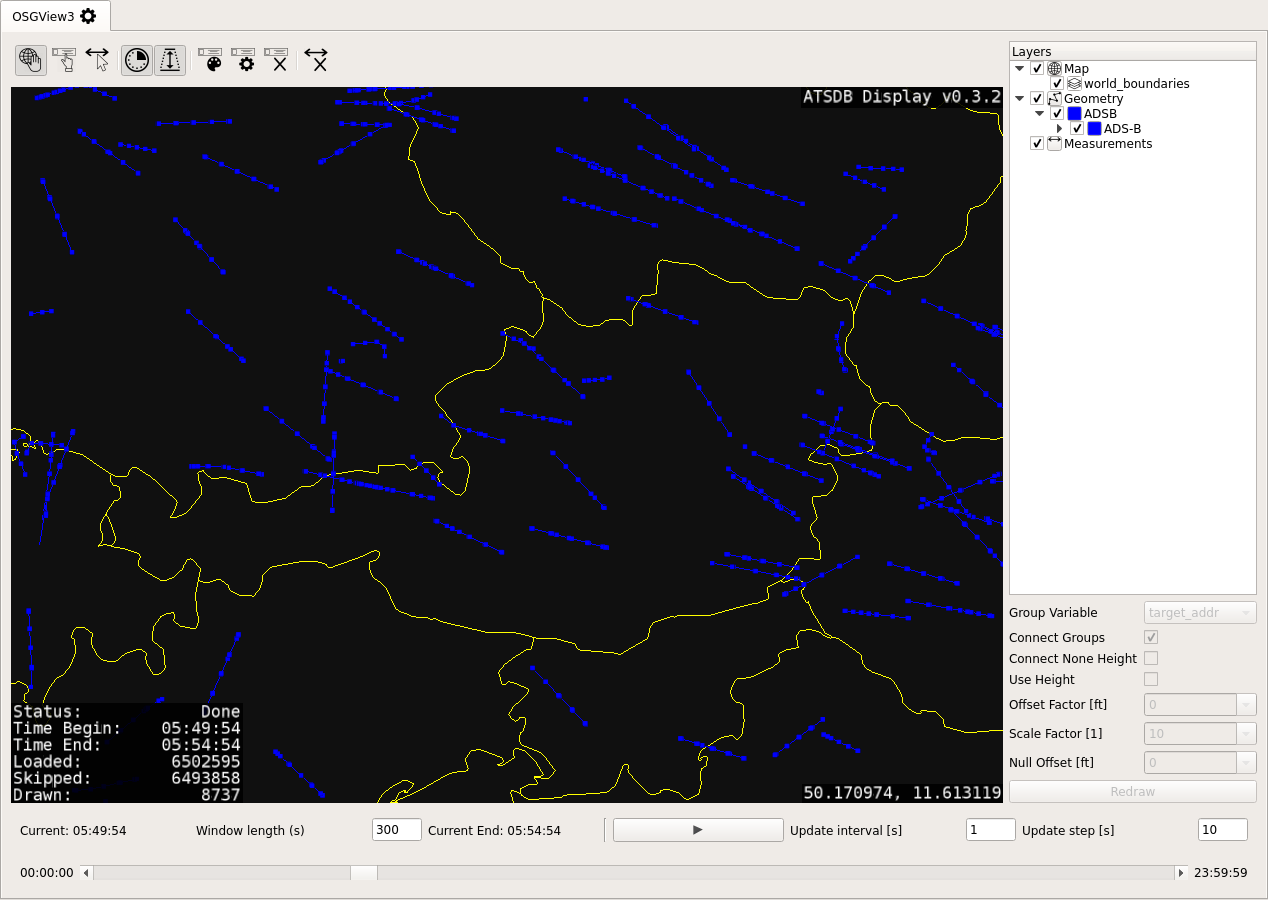
\includegraphics[width=18cm,frame]{../screenshots/osgview_data.png}
  \caption{OSG View data display}
  \label{fig:osgview_data}
\end{figure}

Please note that since currently only an example dataset is used, until real surveillance data can be made available.

Now, the loaded data is displayed in the following manner: For each DBO, a list of sensors exist, which supply the shown target reports. In the Geometry layers, the data is grouped as follows: Database Object $\rightarrow$ Sensor $\rightarrow$ Group. \\

For each DBO, a default display configuration is set:

\begin{itemize}
 \item Tracker: White circle (default)
 \item Radar: Green cross (default)
 \item MLAT: Red triangle (default)
 \item ADS-B: Blue square (default)
\end{itemize}

Please \textbf{note} that the ordering of the layers also reflects the drawing order, especially when the depth check is disabled. This means that the data source 'on top' is drawn over all others. \\

A sensor is of course a defined data source, e.g. a specific radar. A group currently is defined by a track number, and is connected by lines. If no track number is defined, the data is put into the 'Unassociated' group and not connected by lines. \\

Please note that the style (hidden, color, symbol, size etc.) is only persisted for DBO's and their immediate child items (e.g. sensors). 

\subsubsection{Layer Operations}

In the Layers widget, a number of operations are possible for each tree item.

\begin{table}[H]
  \center
  \begin{tabular}{ | l | l | l |}
    \hline
    \textbf{Operation} & \textbf{Trigger} &  \textbf{Description} \\ \hline
    View sub-items & Triangle & Opens or closes view of the sub-items \\ \hline
    Display item & Checkbox & Enables or disables display of items (and all sub-items) \\ \hline
    Display context menu & Click on symbol & Opens the items context menu \\ \hline
  \end{tabular}
  \caption{Layer operations}
\end{table}

The context menu allows several actions to be performed on an item. If an item has sub-items, the same action will automatically be performed on the child items.

\begin{figure}[H]
    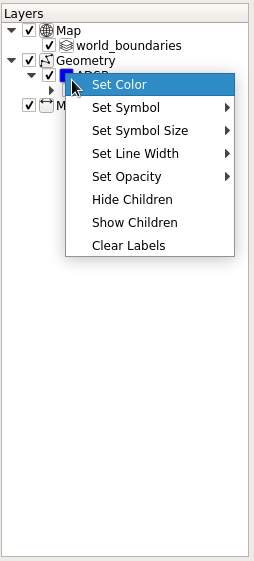
\includegraphics[width=5cm,frame]{../screenshots/osgview_layer_context_menu.png}
  \caption{OSG View layer context menu}
\end{figure}

\paragraph{Special DBO Operations}

\begin{itemize}
 \item Move to Top: Move DBO to first position
 \item Move Up: Move DBO one position up
 \item Move Down: Move DBO one position down
 \item Move to Bottom: Move DBO to the last position
\end{itemize}

The other operations are the same as in the following common operations.

\paragraph{Common Operations}

\begin{itemize}
 \item Set Color: Open colour dialog to set the items colour
 \item Set Symbol: Set the items symbol to one of the following values:
\begin{itemize}
 \item Cross
 \item Circle
 \item Square
 \item Triangle
\end{itemize}
 \item Set Symbol Size: Set the symbols size
 \item Set Line Width: Set the line width
 \item Set Opacity: Set the items opacity
 \item Hide children: Disable display off all children
 \item Show Children: Enable display of all children
 \item Clear Labels: Removes all labels
\end{itemize}

Please note that only the main Map item has a context menu, and only allows setting of map files and changing the opacity.

\subsubsection{Data Labeling}

Labels can be shown for target reports, when the Label mode is active. Simply do a LMB click on a target report symbol.

\begin{figure}[H]
    \hspace*{-2cm}
    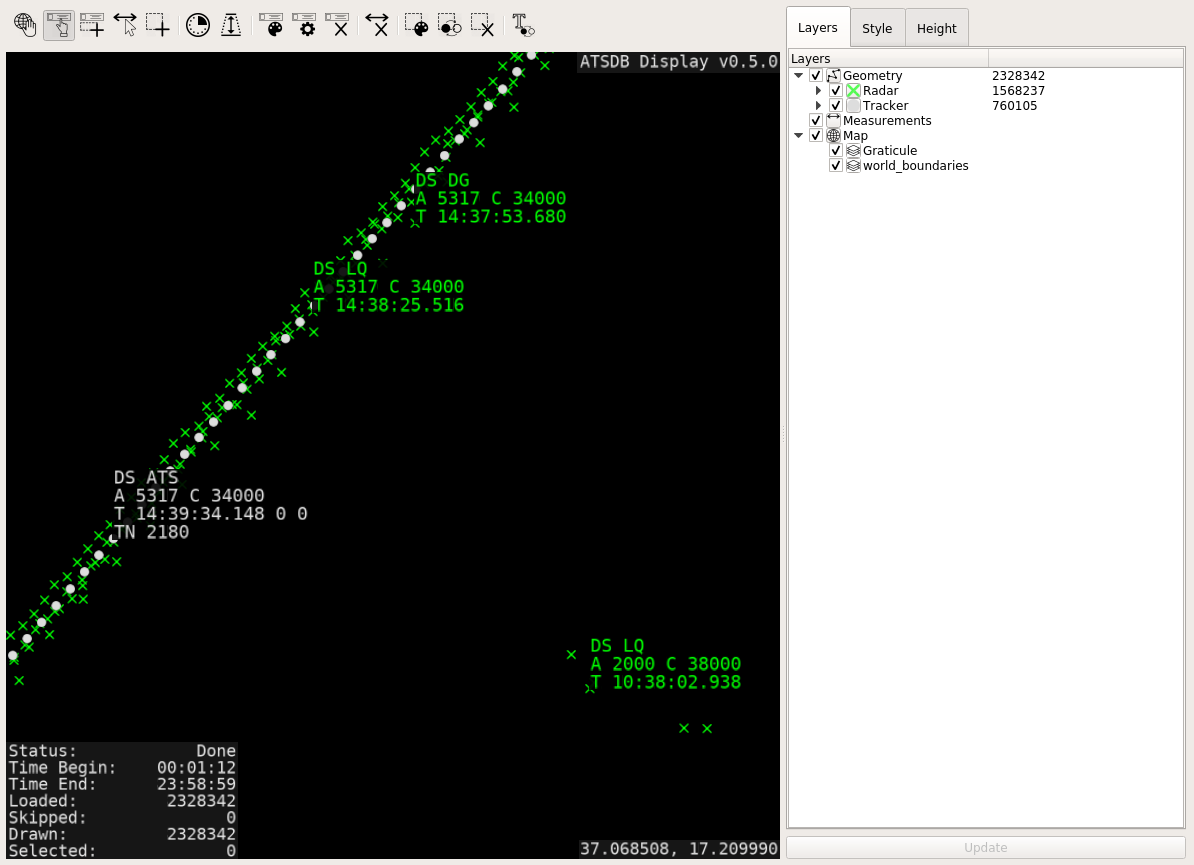
\includegraphics[width=18cm,frame]{../screenshots/osgview_labels.png}
  \caption{OSG View Labels}
\end{figure}

\subsubsection{Geometry Context Menu}

Several data-related operations can be also performed in the map widget when the Label mode is active, by a RMB click on a geometry group.


\begin{figure}[H]
    \hspace*{-2cm}
    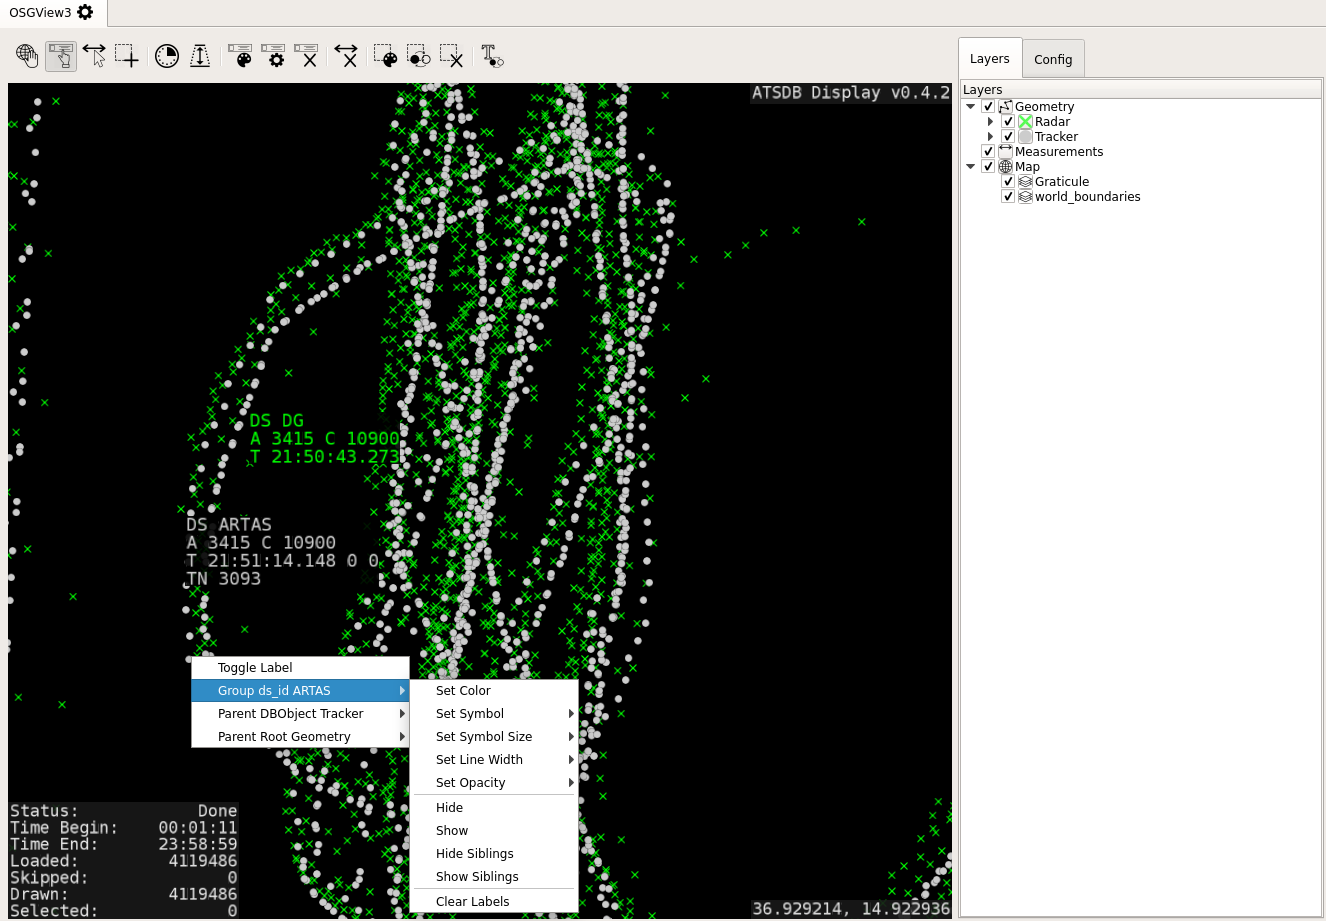
\includegraphics[width=18cm,frame]{../screenshots/osgview_data_operations.png}
  \caption{OSG View data operations}
\end{figure}

The data context menu allows the following operations:

\begin{itemize}
 \item Toogle Label: Toggle label display of a single target report
 \item Group: Same operations as on the item's group layer item
\end{itemize}

\subsubsection{Distance Measurement}

Distance measurements can be made when the Measure mode is active. If 'Use height' is not checked, measurements are done as follows:

Simply do a LMB click on a target report or a position on the map to start the measurement.

\begin{figure}[H]
    \hspace*{-2cm}
    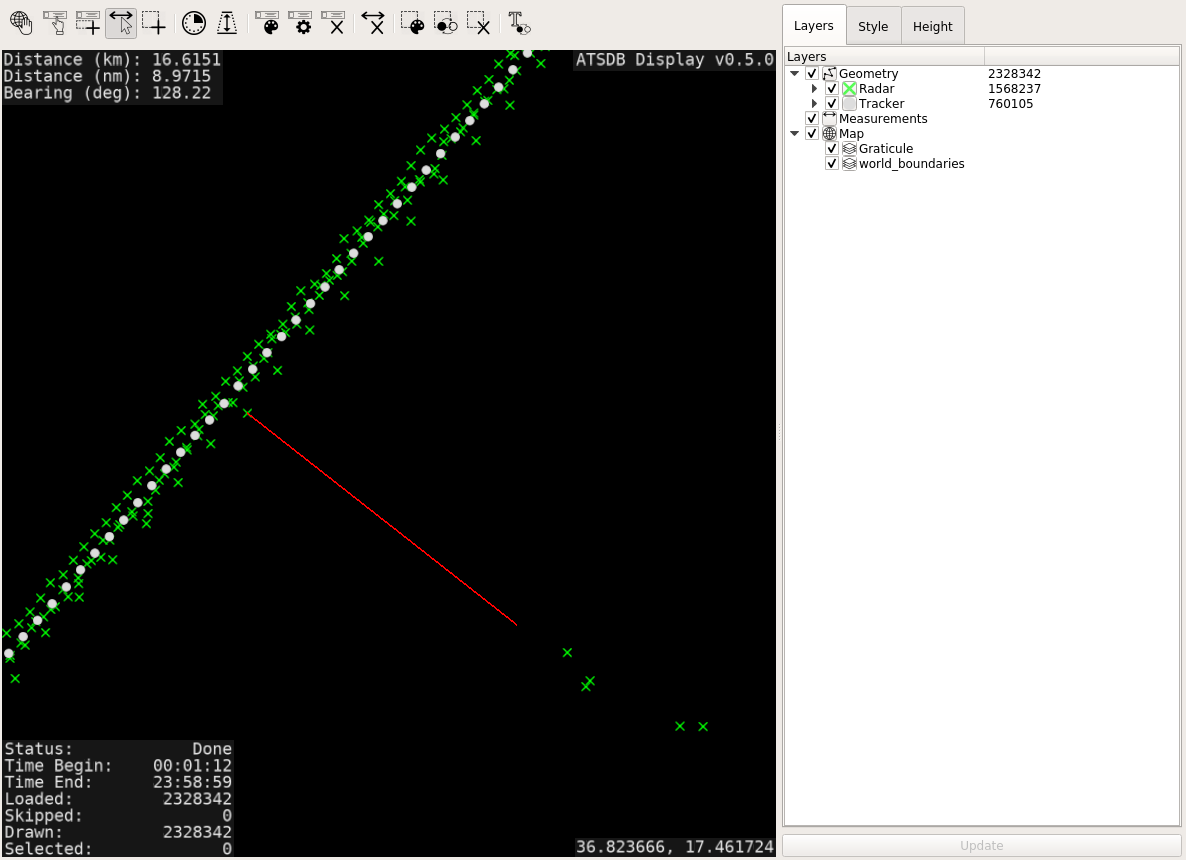
\includegraphics[width=18cm,frame]{../screenshots/osgview_measure1.png}
  \caption{OSG View measurement}
\end{figure}

During the measurement, the following information is shown in the top-left corner:

\begin{itemize}
 \item Distance (km): Great-circle distance using the haversine formula, in meters or kilometers.
 \item Distance (nm): Great-circle distance using the haversine formula, in nautical miles.
 \item  Bearing (deg): Bearing from point 1 to point 2, in degrees from true north.
\end{itemize}

Then do a second LMB click on the map on a point of interest to finish the measurement.

\begin{figure}[H]
    \hspace*{-2cm}
    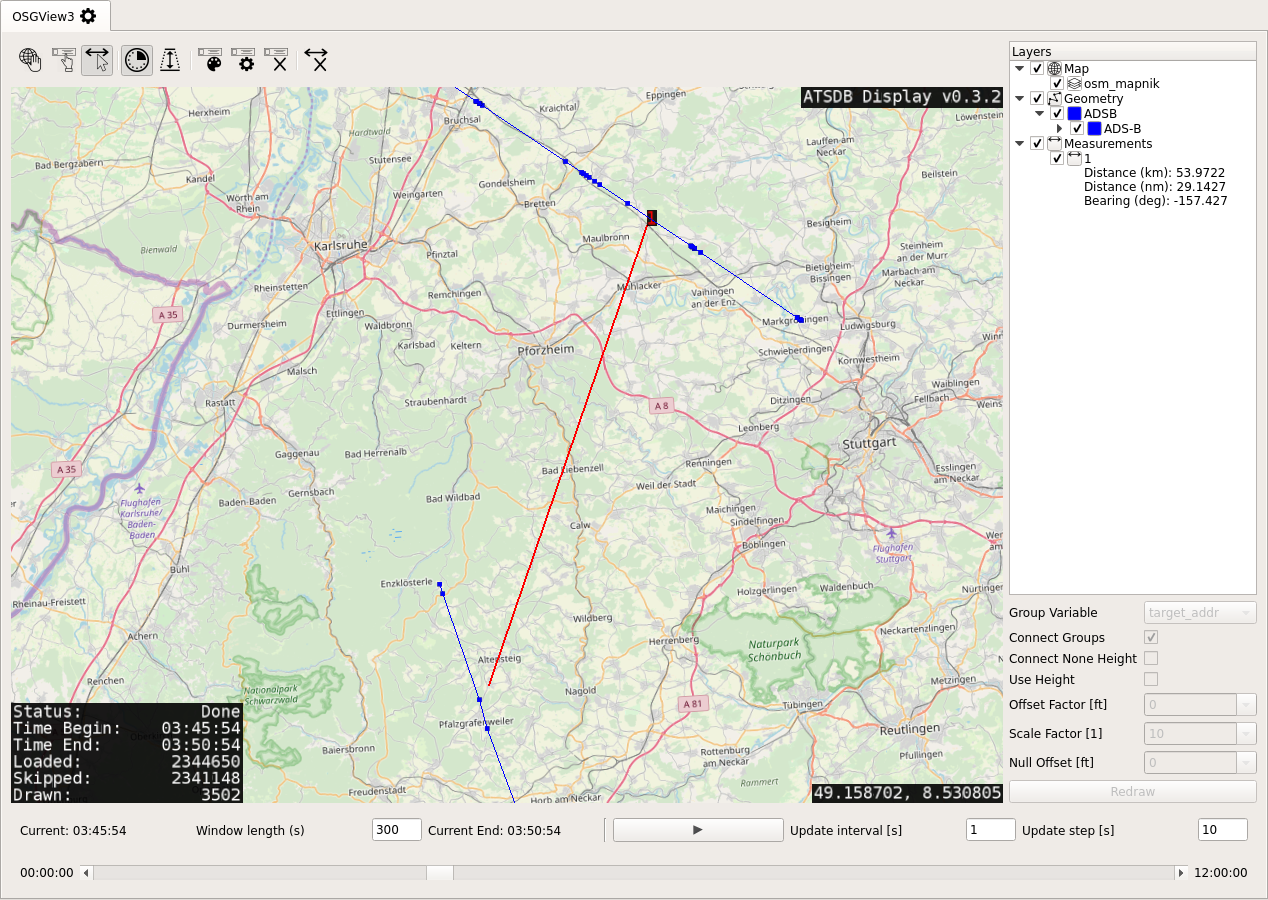
\includegraphics[width=18cm,frame]{../screenshots/osgview_measure2.png}
  \caption{OSG View measurement done}
\end{figure}

If 'Use height' is checked, measurements are calculated in the same way as previously (ground distance), but for each target report with height a connecting line to the respective ground position is displayed. \\

For a measurement between two target reports with height information, the measurement will be displayed as follows:

\begin{figure}[H]
    \hspace*{-2cm}
    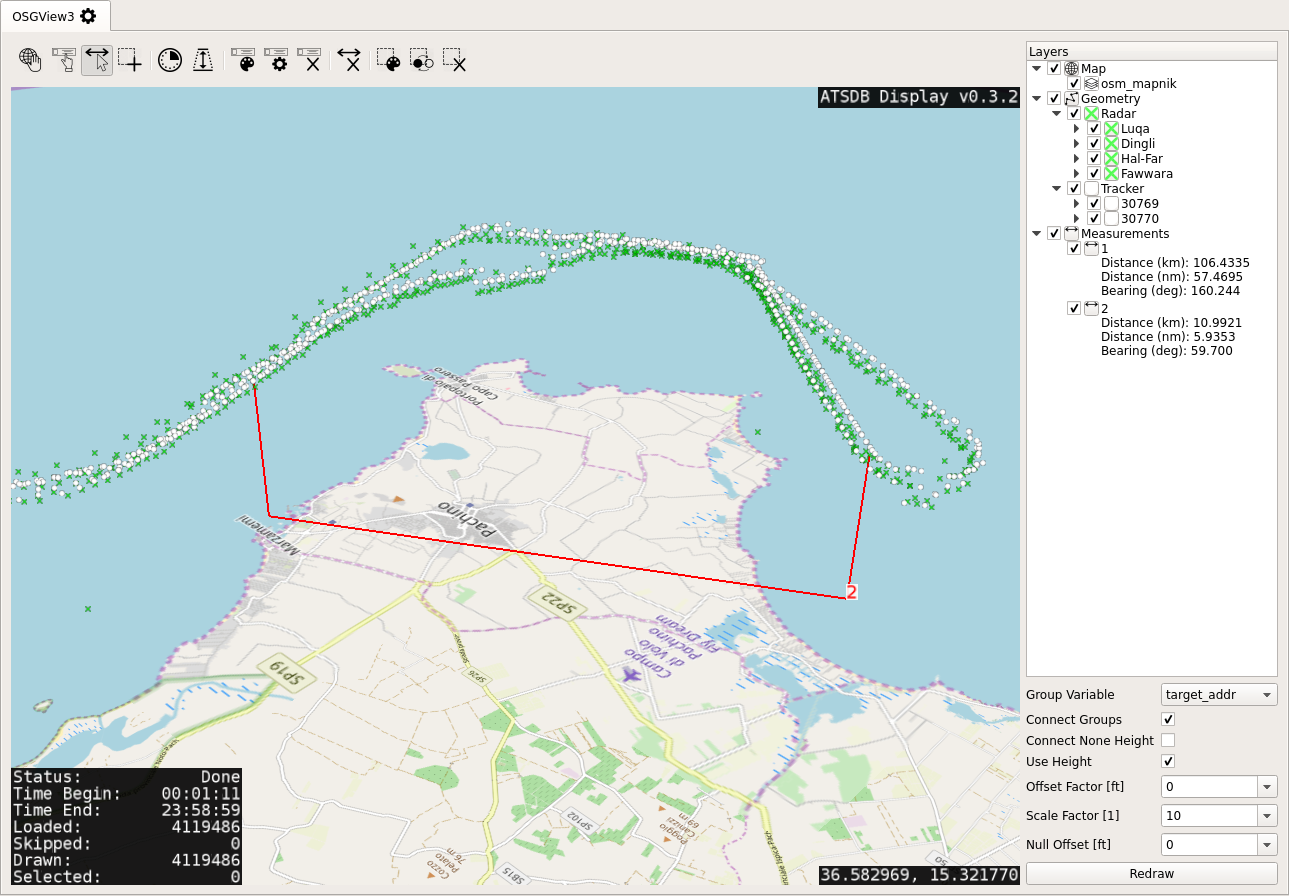
\includegraphics[width=18cm,frame]{../screenshots/osgview_measure3d.png}
  \caption{OSG View measurement with height information}
\end{figure}

The measurements is shown in the Layers tab, and is identified using a number. The visibility for each label can be set using the checkbox, and the layer menu (using the 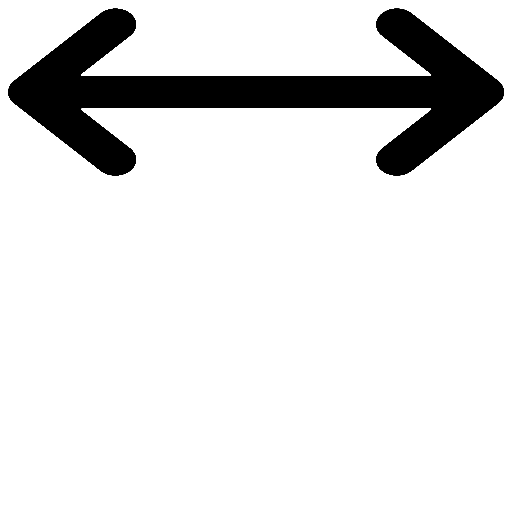
\includegraphics[width=0.5cm]{../../data/icons/measure.png}) symbol) allows the following operations:

\begin{itemize}
 \item Copy text: Copies the text as well as the point information to the clipboard to be pasted in other applications
 \item Delete: Deletes the measurement
\end{itemize}

Please note the the number label background color can be set as with all other labels. 

\subsubsection{Selection}

Target reports can be selected when the Select mode is active. If 'Use height' is not checked, measurements are done as follows:

Simply do a LMB click on a target report or a position on the map to start the selection. Move the mouse to another location to create a red selection rectangle.

\begin{figure}[H]
    \hspace*{-2cm}
    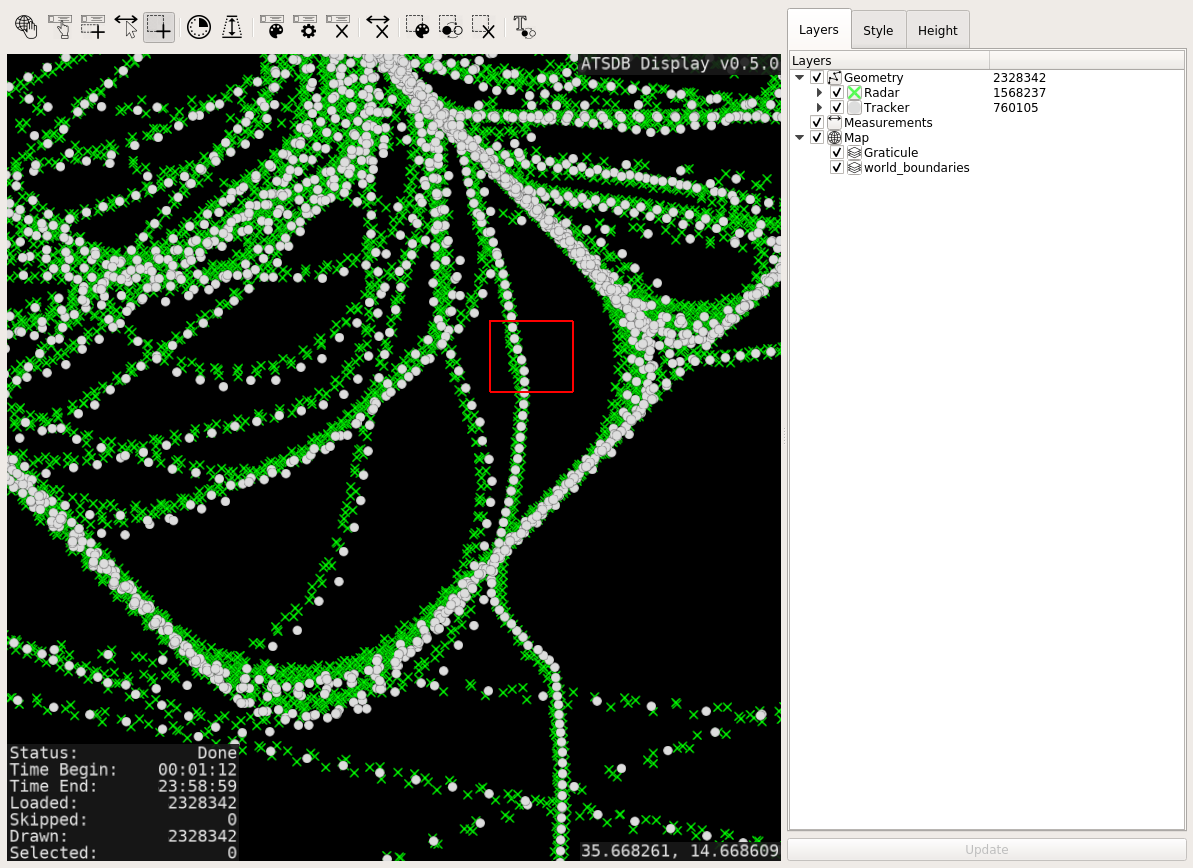
\includegraphics[width=18cm,frame]{../screenshots/osgview_select1.png}
  \caption{OSG View selection}
\end{figure}

With a second LMB click the selection is finalized and all target reports in the created latitude/longitude rectangle are selection. This is shown by a different color (yellow by default), and the 'Selected' counter in the lower-left corner shows the current selection size.

\begin{figure}[H]
    \hspace*{-2cm}
    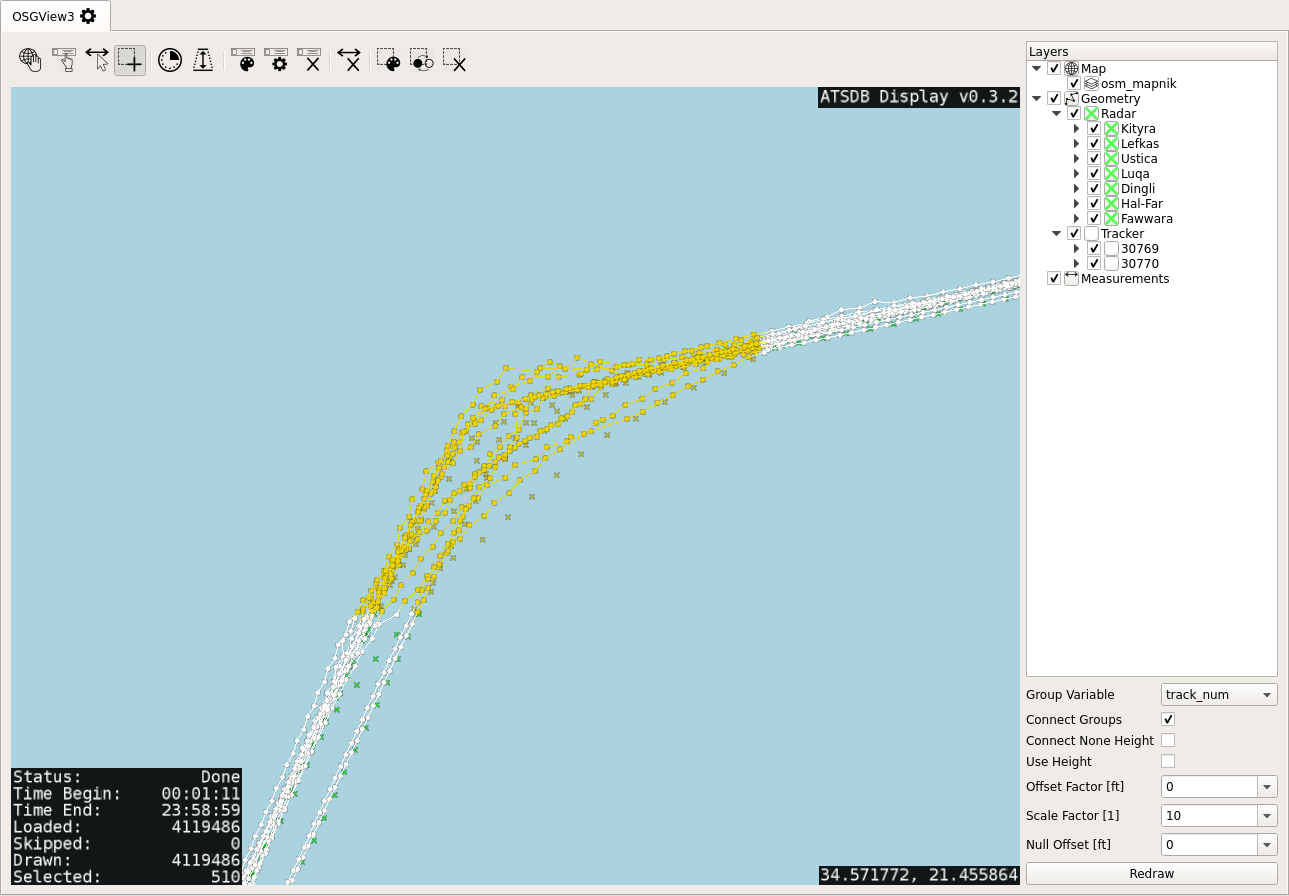
\includegraphics[width=18cm,frame]{../screenshots/osgview_select2.png}
  \caption{OSG View selection done}
\end{figure}

If another selection is done, the previous one is cleared by default. If another selection shown be \textit{added} to the current one, hold down the control key when doing the second LMB click.

\begin{figure}[H]
    \hspace*{-2cm}
    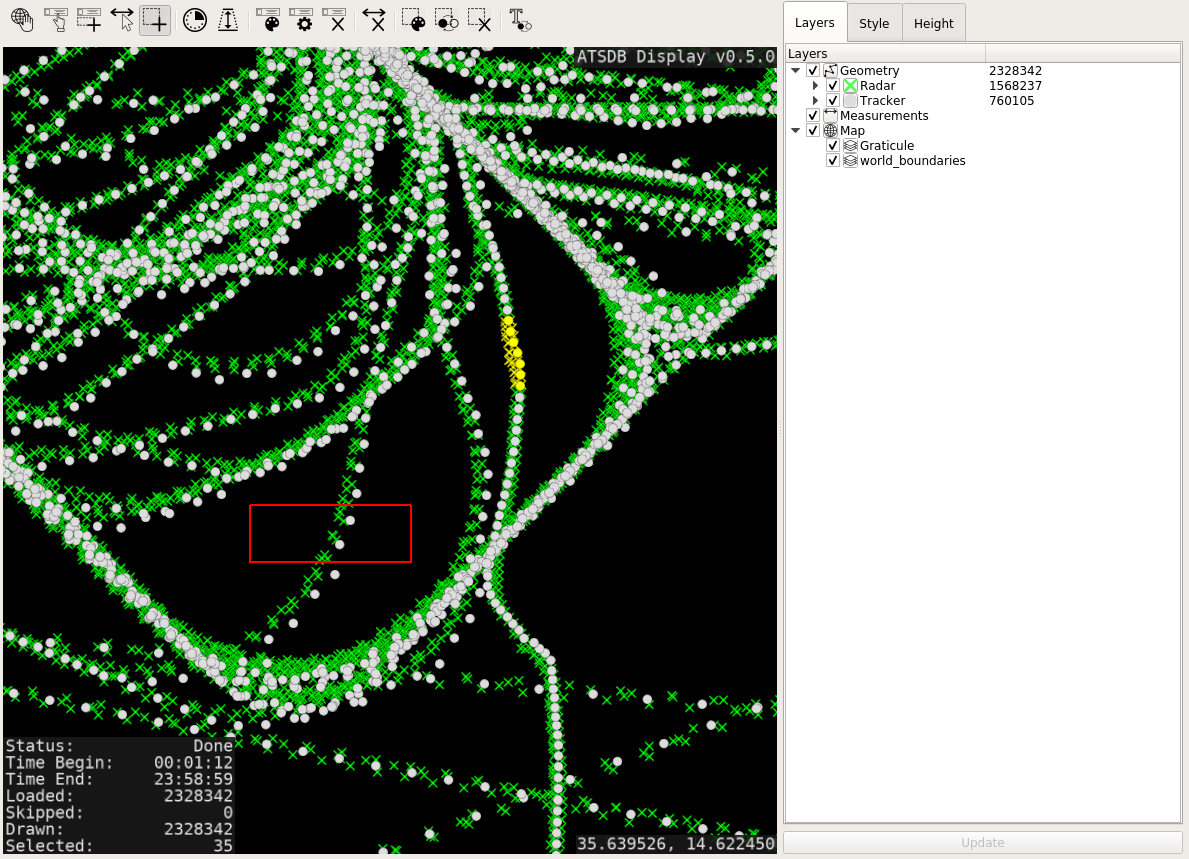
\includegraphics[width=18cm,frame]{../screenshots/osgview_select_add1.png}
  \caption{OSG View selection with adding}
\end{figure}

This adds the target reports within the new red rectangle to the current selecion.

\begin{figure}[H]
    \hspace*{-2cm}
    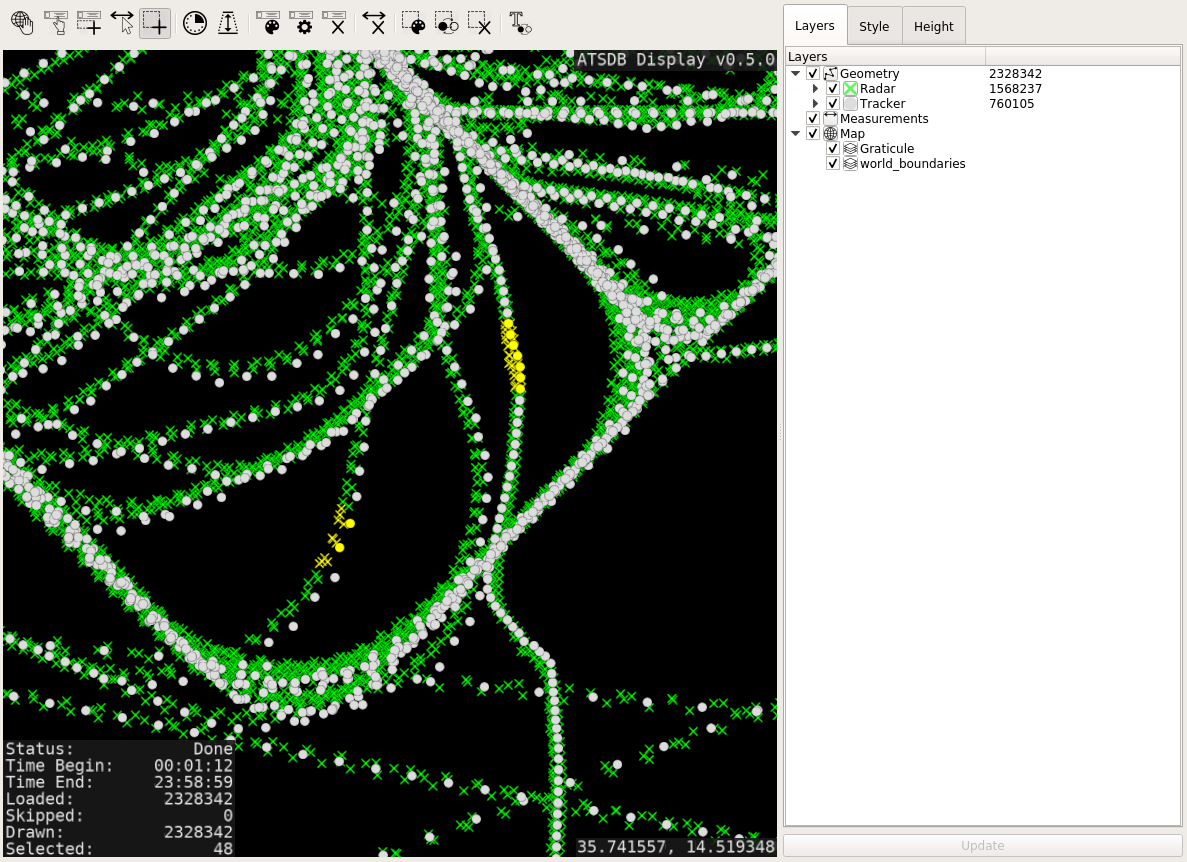
\includegraphics[width=18cm,frame]{../screenshots/osgview_select_add2.png}
  \caption{OSG View selection with adding done}
\end{figure}

If 'Use height' is checked, selection can be done with height information, which is shown as a box. Simply do a LMB click on the map for a target report, and move the cursor to another target report or map location. If both locations have zero height (map location or no height information in target report), again a rectangle is shown. If one or both locations have a non-zero height, a 3D box is displayed.

\begin{figure}[H]
    \hspace*{-2cm}
    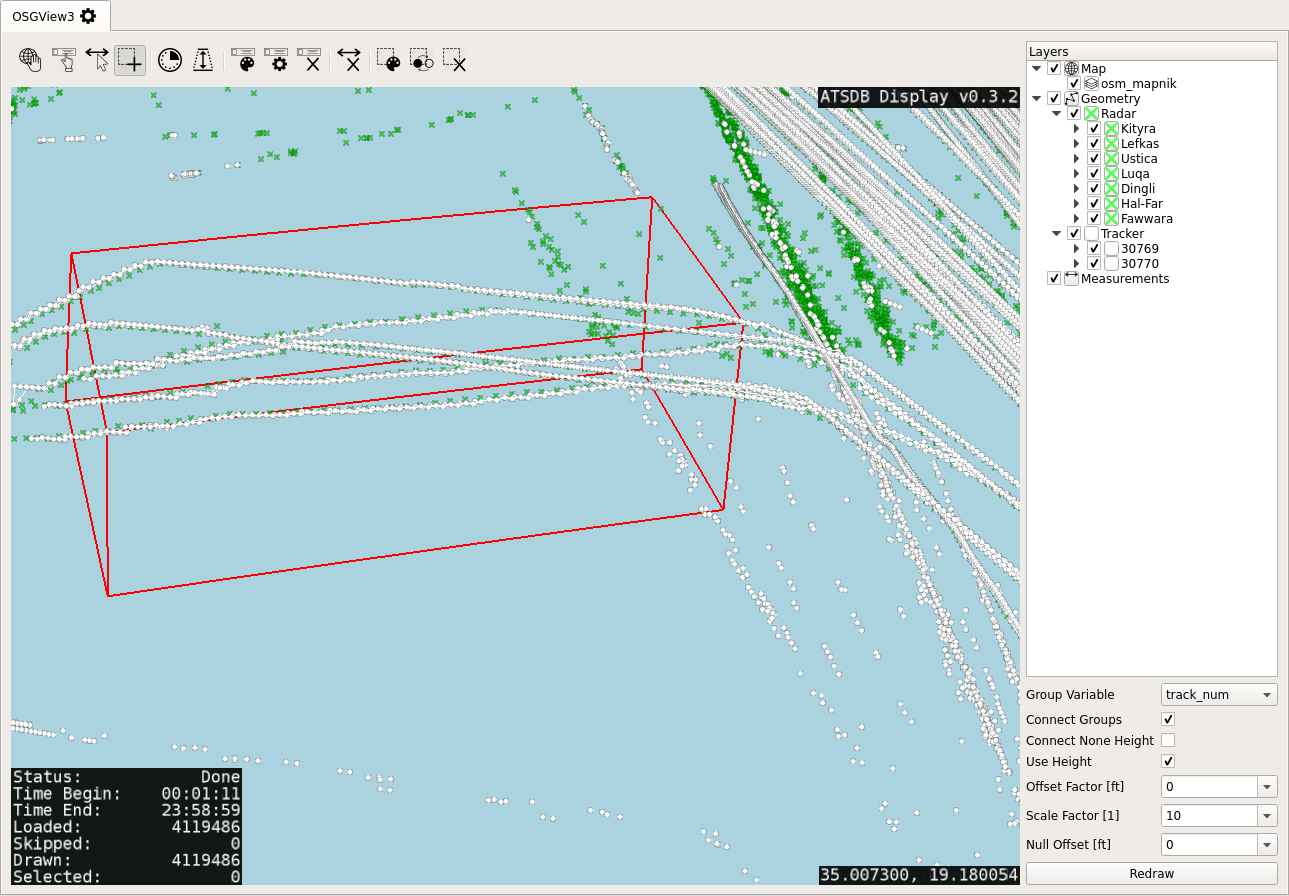
\includegraphics[width=18cm,frame]{../screenshots/osgview_select3d.png}
  \caption{OSG View selection with height}
\end{figure}


\begin{figure}[H]
    \hspace*{-2cm}
    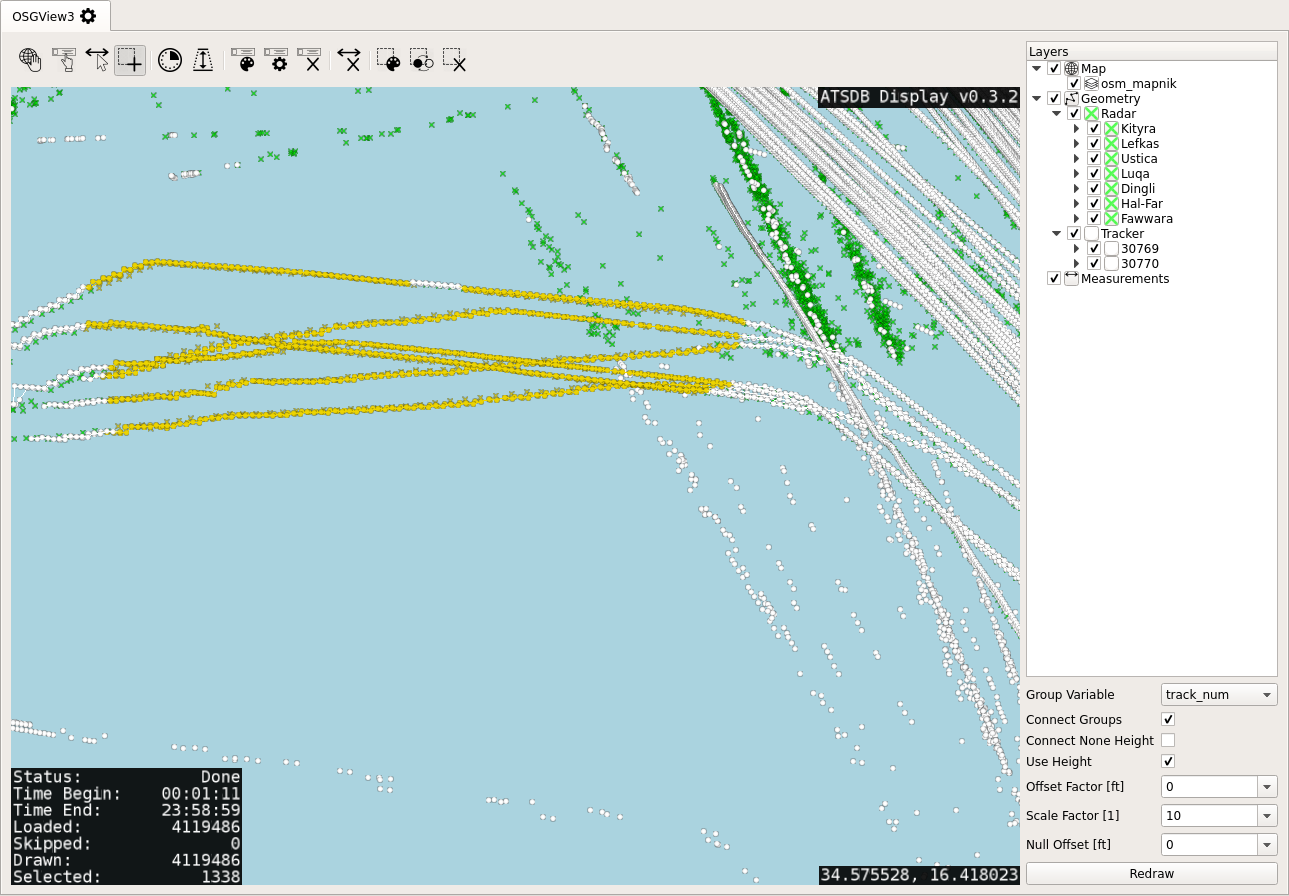
\includegraphics[width=18cm,frame]{../screenshots/osgview_select3d_2.png}
  \caption{OSG View selection with height done}
\end{figure}


\subsubsection{Time Filter}

Once activated using the symbol 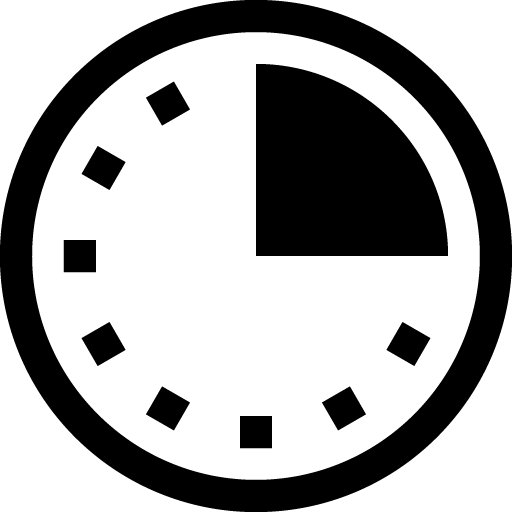
\includegraphics[width=0.5cm]{../../data/icons/time.png} in the toolbar, the time filter facilitates that only target reports within a specific time window are shown.


\begin{figure}[H]
    \hspace*{-2cm}
    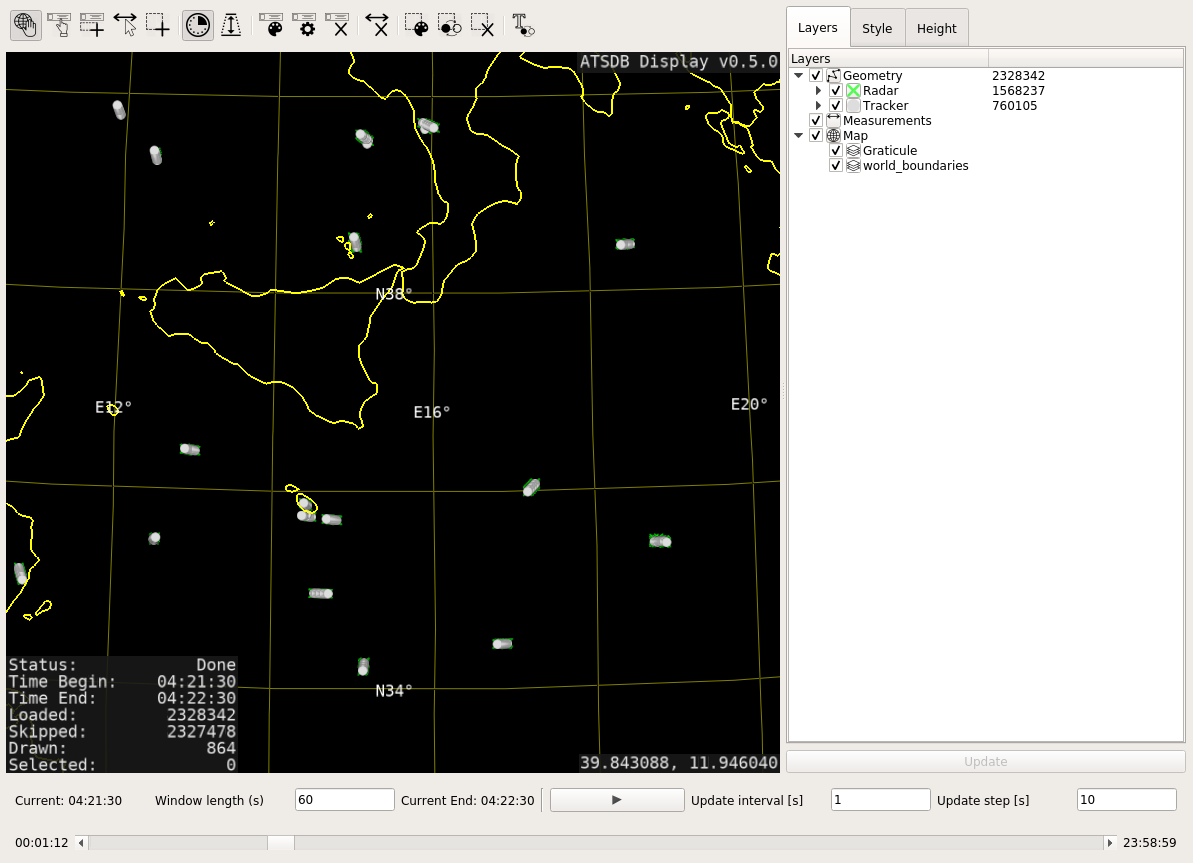
\includegraphics[width=18cm,frame]{../screenshots/osgview_time_filter.png}
  \caption{OSG View time filter}
  \label{fig:osgview_time_filter}
\end{figure}

The following items exist:

\begin{itemize}
 \item Current: The start of the time window
 \item Window length (s): Duration of the display time window
 \item Current End: The end of the time window
 \item Play button: Start/Stop the auto-play mode
 \item Update interval [s]: Auto-play mode update interval
 \item Update step [s]: Auto-play mode update step
 \item Scrollbar: Manual time-scrolling
\end{itemize}

During usage of the time filter, changes in the Configuration Widget was suppressed, but changes in the Layers Widgets are possible.

\subsubsection{Depth Check}

Once activated using the symbol 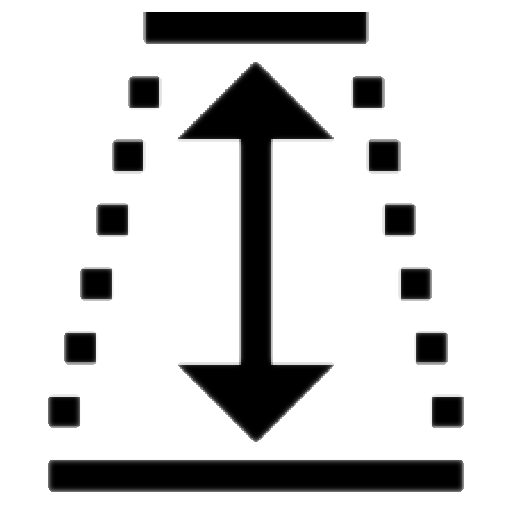
\includegraphics[width=0.5cm]{../../data/icons/depth.png} in the toolbar, during drawing it is checked wether data is occluded in the depicted scene. E.g. if target reports are ``below ground'', they are not shown.

\begin{figure}[H]
    \hspace*{-2cm}
    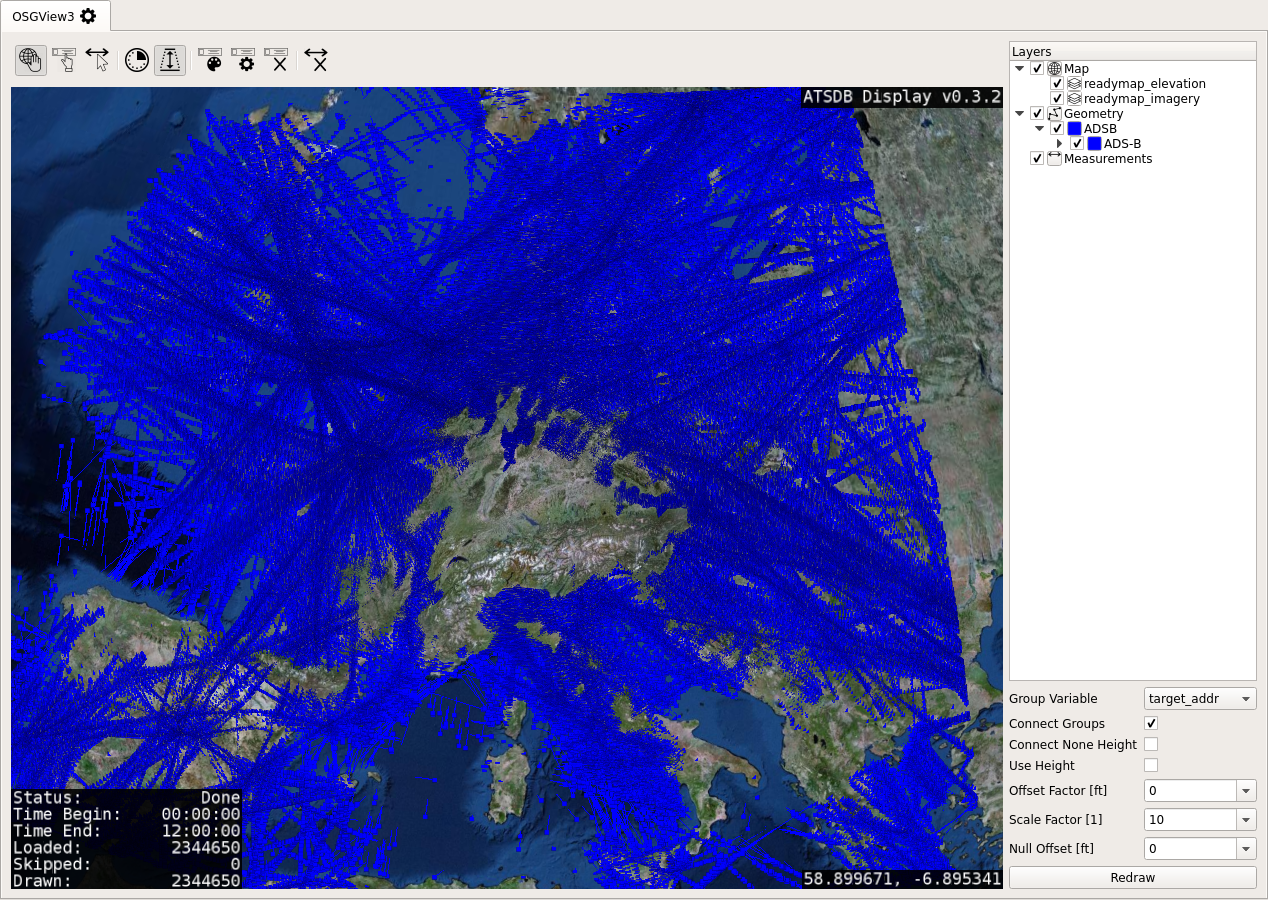
\includegraphics[width=18cm,frame]{../screenshots/osgview_depth_check.png}
  \caption{OSG View depth check}
\end{figure}

\subsubsection{Data Label Background Color}

The background color for existing labels can be configured using the symbol 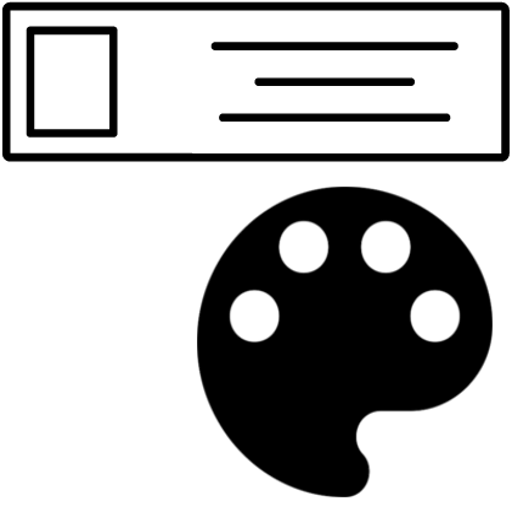
\includegraphics[width=0.5cm]{../../data/icons/label_color.png} in the toolbar.

\subsubsection{Data Label Content Configuration}

Existing labels can be configured using the symbol 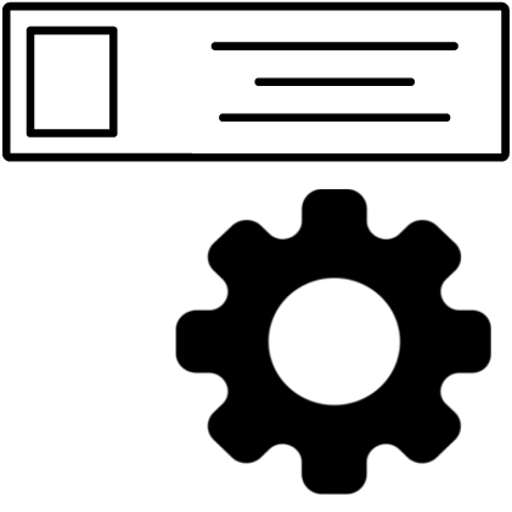
\includegraphics[width=0.5cm]{../../data/icons/label_edit.png} in the toolbar.

The following operations are supported:

\begin{itemize}
 \item Edit: Edits which variables are shown, for each DBO
 \item Line Break: Sets after how many variable entries a line break is used
\end{itemize}

When a edit window for a DBO label definition is opened, a window like the following is shown:

\begin{figure}[H]
    \includegraphics[width=12cm,frame]{../screenshots/osgview_label_edit.png}
  \caption{OSG View Label Editing}
\end{figure}

For each DBO, for each variable it can be selected if the value is presented (using the checkbox), and a prefix and suffix can be defined. The changes made to the prefix and suffix are made by double-clicking on the respective field, entering a new value, and setting the value by pressing enter. Upon each change, the existing labels in the OSG View are updated automatically. \\

A few notes about labels:

\begin{itemize}
 \item The label definition and presentation is persisted in the configuration
 \item The label colour is always the same as the target report's
 \item A variable value is only shown if it is present (not NULL)
 \item Labels are shown at the target reports position, matched to the lower-left corner
 \item A line break is given after the configured number of values. If values are not shown (NULL), the line break is still made at the same postion, to keep the value shown in the same line for all target reports.
\end{itemize}

\subsubsection{Data Label Deletion}

All existing labels can be deleted using the symbol 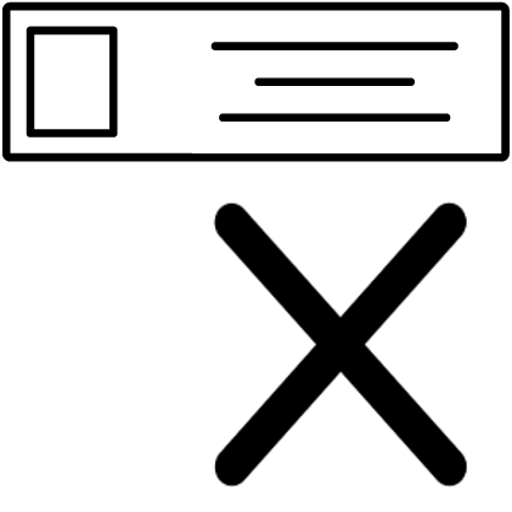
\includegraphics[width=0.5cm]{../../data/icons/label_delete.png} in the toolbar.

\subsubsection{Measurement Deletion}

All existing measurements can be deleted using the symbol 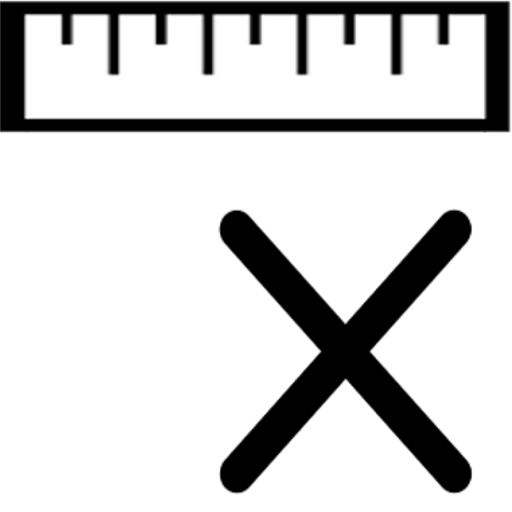
\includegraphics[width=0.5cm]{../../data/icons/measurement_delete.png} in the toolbar.

\subsubsection{Selection Color}

The color for selection highlighting can be configured using the symbol 
\includegraphics[width=0.5cm]{../../data/icons/select_color.png} in the toolbar.

\subsubsection{Selection Invert}

The selection can be inverted using the symbol 
\includegraphics[width=0.5cm]{../../data/icons/select_invert.png} in the toolbar.

\subsubsection{Selection Deletion}

The selection can be erased using the symbol \includegraphics[width=0.5cm]{../../data/icons/select_delete.png} in the toolbar.

\subsubsection{Overlay Text Color Invert}

The overlay text color can be toggled between black on white or white on black using the symbol \includegraphics[width=0.5cm]{../../data/icons/text_invert.png} in the toolbar. Depending on the map background one or the other is more suitable.

\subsubsection{Group Variable}

In this selectection the Meta DBOVariable used to create groups can be changed. Currently, only track number and Mode S address are supported. If e.g. data is shown, that has no track number but a Mode S address, this can be used to connect the respective targets.

\begin{figure}[H]
    \hspace*{-2cm}
    \includegraphics[width=18cm,frame]{../screenshots/osgview_group_variable.png}
  \caption{OSG View group variable}
\end{figure}


\subsubsection{Group Lines}

Grouping is currently performed on track number. If the ``Connect Groups'' checkbox is set, connection lines between all target reports in the same group are drawn, except for the ``Unassociated group'', where not track number was set.

\begin{figure}[H]
    \hspace*{-2cm}
    \includegraphics[width=18cm,frame]{../screenshots/osgview_no_lines.png}
  \caption{OSG View Data without lines}
\end{figure}

If the height information is used (3D view), if target reports without height information are connected, the lines clutter the display. The ``Connect None Height'' checkbox allows to set the behaviour. \\

Please \textbf{note} that changes both these values requires a manual redraw using the ``Redraw'' button.

\subsubsection{Height Operations}

Per default, a target reports height is not used for display, which is common in current air-traffic displays. However, in certain situation a true 3D display might be of interest to a user, and therefore several options where incorporated:

\begin{itemize}
 \item Use Height: Use the height based on Mode C $h_c$, transformed to meters
 \item Offset Factor: If height information is used, this factor $h_o$ is added to the height
 \item Scale Factor: If height information is used, this factor $h_s$ is used to multiply the height
 \item Null Offset: If height information is used, this factor $h_n$ is used for target reports without height information
\end{itemize}

Generally, if no height information is given (no Mode C code), the height is either $0$ or the height offset (if used). That means that those target reports appear to the on the ground. If connection lines are drawn between the ones in the air and those without, a lot of annoying lines are shown.

The formula to calculate the height (if existing) is as follows:

$$ h = h_o + h_s \cdot h_c [m]$$ 

If no height information is given:

$$ h = h_n [m]$$ 

Please note that upon changes to the height usage, a manual redraw has to be performed using the ``Redraw'' button.


\begin{figure}[H]
    \hspace*{-2cm}
    \includegraphics[width=18cm,frame]{../screenshots/osgview_use_height.png}
  \caption{OSG View use height}
\end{figure}

 
